
%%%%%%%%%%%%%%%%%%%%%%%%%%%%%%%%%%%%%%%%%%%%%%%%%%%%%%%%%%%%%%%%%%%%%%%%%%%%%%%
\chapter{Lipschitz Bound of Convolutional Neural Network}
\label{chapter:lipschitz_bound}
%%%%%%%%%%%%%%%%%%%%%%%%%%%%%%%%%%%%%%%%%%%%%%%%%%%%%%%%%%%%%%%%%%%%%%%%%%%%%%%
\localtableofcontents

% \begin{abstract}
% This paper tackles the problem of Lipschitz regularization of Convolutional Neural Networks. Lipschitz regularity is now established as a key property of modern deep learning with implications in training stability, generalization, robustness against adversarial examples, etc. However, computing the exact value of the Lipschitz constant of a neural network is known to be NP-hard. Recent attempts from the literature introduce upper bounds to approximate this constant that are either efficient but loose or accurate but computationally expensive. In this work, by leveraging the theory of Toeplitz matrices, we introduce a new upper bound for convolutional layers that is both tight and easy to compute. Based on this result we devise an algorithm to train Lipschitz regularized Convolutional Neural Networks.
% \end{abstract}


%%%%%%%%%%%%%%%%%%%%%%%%%%%%%%%%%%%%%%%%%%%%%%%%%%%%%%%%%%%%%%%%%%%%%%%%%%%%%%%
\section{Introduction}
\label{section:ch4-introduction}
%%%%%%%%%%%%%%%%%%%%%%%%%%%%%%%%%%%%%%%%%%%%%%%%%%%%%%%%%%%%%%%%%%%%%%%%%%%%%%%


The last few years have witnessed a growing interest in Lipschitz regularization of neural networks, with the aim of improving their generalization~\cite{bartlett2017spectrally}, their robustness to adversarial attacks~\cite{tsuzuku2018lipschitz, farnia2018generalizable}, or their generation abilities (\eg for GANs: \cite{miyato2018spectral,arjovsky2017wasserstein}).
Unfortunately computing  the exact Lipschitz constant of a neural network is NP-hard~\cite{scaman2018lipschitz} and in practice, existing techniques such as~\cite{scaman2018lipschitz, NIPS2019_9319} or~\cite{latorre2020lipschitz} are difficult to implement for neural networks with more than one or two layers, which hinders their use in deep learning applications.

To overcome this difficulty, most of the work has focused on computing the Lipschitz constant of {\em individual layers} instead.
The product of the Lipschitz constant of each layer is an upper-bound for the Lipschitz constant of the entire network, and it can be used as a surrogate to perform Lipschitz regularization.
Since most common activation functions (such as ReLU) have a Lipschitz constant equal to one, the main bottleneck is to compute the Lipschitz constant of the underlying linear application which is equal to its maximal singular value.
The work in this line of research mainly relies on the celebrated iterative algorithm by~\citet{golub2000eigenvalue} used to approximate the maximum singular value of a linear function.
Although generic and accurate, this technique is also computationally expensive, which impedes its usage in large training settings. 

In this paper we introduce a new tight and easy to compute  upper bound on the largest singular value of convolution layers.
We rely on Toeplitz matrix theory and its links with Fourier analysis.
It is known that the sequence of elements that characterizes a Toeplitz matrix is the Fourier transform of a given trigonometric polynomial.
We extend this result to doubly-block Toeplitz matrices (\ie block Toeplitz matrices where each block is Toeplitz) and devise a bound on the singular values of these matrices as a function of a multivariate trigonometric polynomial.
Implementing this bound in the context of convolutional neural networks, requires further to consider a sequence of doubly-block Toeplitz matrices, since the entries are commonly chosen to be tensors of more than one dimension.
As a main result, we devise an upper bound for a stacked sequence of doubly-block Toeplitz matrices, which fits well the requirements of CNNs, both in terms of applicability and efficiency.
From our analysis immediately follows an algorithm for bounding the Lipschitz constant of a convolutional layer, and by extension the Lipschitz constant of the whole network. 

Finally, we illustrate our approach on adversarial robustness.
Recent work has shown that empirical methods such as adversarial training offer poor generalization~\cite{schmidt2018adversarially}, and can be improved by applying Lipschitz regularization~\cite{farnia2018generalizable}.
To illustrate the benefit of our new method, we train a large, state-of-the-art Wide ResNet architecture with Lipschitz regularization and show that it offers a significant improvement over adversarial training alone, and over other methods for Lipschitz regularization.
To sum up, we make the following  contributions:
\begin{enumerate}
    \item We devise an upper bound on the singular values of the operator matrix of convolutional layers by leveraging Toeplitz matrix theory and its links with Fourier analysis. 
    \item We propose an efficient algorithm to compute this upper bound which enables its use in the context of convolutional neural networks.
    \item We use our method to regularize the Lipschitz constant of neural networks in the area of adversarial robustness and show that it offers a significant improvement over adversarial training alone.
\end{enumerate}

%%%%%%%%%%%%%%%%%%%%%%%%%%%%%%%%%%%%%%%%%%%%%%%%%%%%%%%%%%%%%%%%%%%%%%%%%%%%%%%
\section{Related Work}
\label{section:ch4-related_work}
%%%%%%%%%%%%%%%%%%%%%%%%%%%%%%%%%%%%%%%%%%%%%%%%%%%%%%%%%%%%%%%%%%%%%%%%%%%%%%%

A popular technique for approximating the maximal singular value of a matrix is the power method~\cite{golub2000eigenvalue}, an iterative algorithm which yields a good approximation of the maximum singular value when the algorithm is able to run for a sufficient number of iterations. 
\citet{yoshida2017spectral, miyato2018spectral} have used the power method to normalize the spectral norm of each layer of a neural network, and showed that the resulting models offered improved generalization performance and generated better examples when they were used in the context of GANs. 
\citet{farnia2018generalizable} built upon the work of~\citet{miyato2018spectral} and proposed a power method specific for convolutional layers that leverages the deconvolution operation and avoid the computation of the gradient.
They used it in combination with adversarial training. 
In the same vein, \citet{gouk2018regularisation} demonstrated that regularized neural networks using the power method also offered improvements over their non-regularized counterparts. 
Furthermore, \citet{tsuzuku2018lipschitz} have shown that a neural network can be more robust to some adversarial attacks, if the prediction margin of the network (\ie the difference between the first and the second maximum logit) is higher than a minimum threshold that depends on the global Lipschitz constant of the network.
Building on this observation, they use the power method to compute an upper bound on the global Lipschitz constant, and maximize the prediction margin during training.
Finally, \citet{scaman2018lipschitz} have used automatic differentiation combined with the power method to compute a tighter bound on the global Lipschitz constant of neural networks.
Despite a number of interesting results, using the power method is expensive and results in prohibitive training times. 

Other approaches to regularize the Lipschitz constant of neural networks have been proposed by~\citet{sedghi2018iclr} and~\citet{singla2019bounding}.
The method of~\citet{sedghi2018iclr} exploits the properties of circulant matrices to approximate the maximal singular value of a convolutional layer.
Although interesting, this method results in a loose approximation of the maximal singular value of a convolutional layer.
Furthermore, the complexity of their algorithm is dependent on the convolution input which can be high for large datasets such as ImageNet.
More recently, \citet{singla2019bounding} have successfully bounded the operator norm of the Jacobian matrix of a convolution layer by the Frobenius norm of the reshaped kernel.
This technique has the advantage to be very fast to compute and to be independent of the input size but it also results in a loose approximation. 

To build robust neural networks, \citet{cisse2017parseval} and ~\citet{NIPS2019_9673} have proposed to constrain the Lipschitz constant of neural networks by using orthogonal convolutions.
\citet{cisse2017parseval} use the concept of \emph{parseval tight frames}, to constrain their networks.
\citet{NIPS2019_9673} built upon the work of~\citet{cisse2017parseval} to propose an efficient construction method of orthogonal convolutions.  

Finally, recent work~\citet{NIPS2019_9319,latorre2020lipschitz} has proposed a tight bound on the Lipschitz constant of the full network with the use of semi-definite programming.
These works are theoretically interesting but lack scalability (\ie the bound can only be computed on small networks).


%%%%%%%%%%%%%%%%%%%%%%%%%%%%%%%%%%%%%%%%%%%%%%%%%%%%%%%%%%%%%%%%%%%%%%%%%%%%%%%
\section{A Primer on Toeplitz and block Toeplitz matrices}
\label{section:primer_toeplitz_matrix}
%%%%%%%%%%%%%%%%%%%%%%%%%%%%%%%%%%%%%%%%%%%%%%%%%%%%%%%%%%%%%%%%%%%%%%%%%%%%%%%

\subsection{Convolution as Matrix Multiplication}\label{section:conv_matrix_multiplication}

A discrete convolution between a signal $\mathbf{x}$ and a kernel $\mathbf{k}$ can be expressed as a  product between the vectorization of $\mathbf{x}$ and a doubly-block Toeplitz matrix $\textbf{M}$, whose coefficients have been chosen to match the convolution $\mathbf{x} * \mathbf{k}$.
For a 2-dimensional signal $\mathbf{x} \in \mathbb{R}^{n \times n}$ and a kernel $\mathbf{k} \in \mathbb{R}^{m \times m}$ with $m$ odd, the convolution operation can be written as follows:
\begin{equation} \label{equation:equation_conv_as_matrix}
    \reshape(\mathbf{y}) = \reshape(\pad(\mathbf{x}) * \mathbf{k}) = \Mmat \reshape(\mathbf{x})
\end{equation}
where $\Mmat$ is a $n^2$-by-$n^2$  doubly-block Toeplitz matrix, \ie a block Toeplitz matrix where the blocks are also Toeplitz (Note that this is not a doubly-block circulant matrix because of the padding.), $\mathbf{y}$ is the output of size $q \times q$ with $q = n - m + 2p + 1$, (see \eg \cite{dumoulin2016guide}).
The $\reshape: \mathbb{R}^{n \times n} \rightarrow \mathbb{R}^{n^2}$ operator is defined as follows: $\reshape(\mathbf{x})_q = \mathbf{x}_{\lfloor q/n \rfloor,\ q\mod n}$.
The $\pad: \mathbb{R}^{n \times n} \rightarrow \mathbb{R}^{(n+2p) \times (n+2p)}$ operator is a zero-padding operation which takes a signal $\mathbf{x}$ of shape $\mathbb{R}^{n \times n}$ and adds $0$ on the edges so as to obtain a new signal $\mathbf{y}$ of shape $\mathbb{R}^{(n+2p) \times (n+2p)}$.
In order to have the same shape between the convoluted signal and the signal, we set $ p = \lfloor m/2 \rfloor$ \footnote{We take a square signal and an odd size square kernel to simplify the notation but the same applies for any input and kernel size.
Also, we take a specific padding in order to have the same size between the input and output signal.
But everything in the paper can be generalized to any paddings.}.

We now present an example of the convolution operation with doubly-block Toeplitz matrix.
Let us define a kernel $\mathbf{k} \in \mathbb{R}^{3\times3}$ as follows:
\begin{equation}
    \mathbf{k} = \begin{pmatrix}
        k_{0} & k_{1} & k_{2} \\
        k_{3} & k_{4} & k_{5} \\
        k_{6} & k_{7} & k_{8} 
    \end{pmatrix}
\end{equation}
If we set the padding to 1, then, the matrix $\Mmat$ is a tridiagonal doubly-block Toeplitz matrix of size $n \times n$ and has the following form:
\begin{equation}
    \Mmat = \begin{pmatrix}
    \Tmat_0 & \Tmat_{1} &  &  & 0  \\
    \Tmat_{2} & \Tmat_0 & \Tmat_{1} &  &  \\
     & \Tmat_{2} & \scalebox{.70}{$\ddots$} & \scalebox{.70}{$\ddots$} &   \\
     &  & \scalebox{.70}{$\ddots$} & \Tmat_0 & \Tmat_{1}  \\
    0 &  &  & \Tmat_{2} & \Tmat_0  \\
    \end{pmatrix}
    \label{equation:operator_matrix}
\end{equation}

where $\Tmat_j$ are banded Toeplitz matrices and the values of $\mathbf{k}$ are distributed in the Toeplitz blocks as follow:
\begin{align}
\Tmat_0 = \begin{psmallmatrix}
    k_{4} & k_{3} &  &  &  0 \\
    k_{5} & k_{4} & k_{3} &  &   \\
     & k_{5} & \scalebox{.40}{$\ddots$} & \scalebox{.40}{$\ddots$}  \\
     &  &  \scalebox{.40}{$\ddots$} & k_{4} & k_{3}  \\
    0 &  &  & k_{5} & k_{4}  \\
    \end{psmallmatrix} &&
\Tmat_{1} = \begin{psmallmatrix}
    k_{7} & k_{6} &  &  &  0 \\
    k_{8} & k_{7} & k_{6} &  &   \\
     & k_{8} & \scalebox{.40}{$\ddots$} & \scalebox{.40}{$\ddots$} &    \\
     &  &  \scalebox{.40}{$\ddots$} & k_{7} & k_{6}  \\
    0 &  &  & k_{8} & k_{7}  \\
    \end{psmallmatrix} &&
\Tmat_{2} = \begin{psmallmatrix}
    k_{1} & k_{0} &  &  &  0 \\
    k_{2} & k_{1} & k_{0} &  &   \\
     & k_{2} & \scalebox{.40}{$\ddots$} & \scalebox{.40}{$\ddots$} &    \\
     &  &  \scalebox{.40}{$\ddots$} & k_{1} & k_{0}  \\
    0 &  &  & k_{2} & k_{1}  \\
    \end{psmallmatrix} 
\end{align}


\paragraph{Remark 1: } Note that the size of the operator matrix $\Mmat$ of a convolution operation depends on the size of the signal. If a signal $\mathbf{x}$ has size $n \times n$, the vectorized signal will be of size $n^2$ and the operator matrix will be of size $n^2 \times n^2$ which can be very large. Indeed, in deep learning practice the size of the images used for training can range from 32 (CIFAR-10) to hundred for high definition images (ImageNet). Therefore, with classical methods, computing the singular values of this operator matrix can be very expensive.

\paragraph{Remark 2: } In the particular case of zero padding convolution operation, the operator matrix is a Toeplitz block with circulant block (i.e. each block of the Toeplitz block is a circulant matrix) which is a particular case of doubly-block Toeplitz matrices. 


\subsection{Generating a Toeplitz matrix and block Toeplitz matrix from a trigonometric polynomial}
An $n\times n$ Toeplitz matrix $\mathbf A$ is fully determined by a two-sided sequence of scalars: $\{a_\seqidx\}_{\seqidx \in \seqsetN}$, whereas an $nm\times nm$ block Toeplitz matrix $\Bmat$ is fully determined by a two-sided sequence of blocks $\{\Bmat_\seqidx\}_{\seqidx \in \seqsetN}$ and where each block $\Bmat_\seqidx$ is an $m \times m$ matrix.  

% \begin{equation}
%     \Amat \triangleq  \begin{psmallmatrix}
%       a_0 & a_{1}   & a_{2} & \cdots & \cdots & a_{n-1}  \\
%       a_{-1} & a_0 & a_{1} & \ddots & & \vdots \\
%       a_{-2} & a_{-1} & \ddots & \ddots & \ddots & \vdots \\ 
%      \vdots & \ddots & \ddots & \ddots & a_{1} & a_{2}\\
%      \vdots & & \ddots & a_{-1} & a_{0} & a_{1} \\
%     a_{-n+1} & \cdots & \cdots & a_{-2} & a_{-1} & a_0
%     \end{psmallmatrix} \quad \quad
%     \Bmat \triangleq  \begin{psmallmatrix}
%       \Bmat_0 & \Bmat_{1}   & \Bmat_{2} & \cdots & \cdots & \Bmat_{n-1}  \\
%       \Bmat_{-1} & \Bmat_0 & \Bmat_{1} & \ddots & & \vdots \\
%       \Bmat_{-2} & \Bmat_{-1} & \ddots & \ddots & \ddots & \vdots \\ 
%      \vdots & \ddots & \ddots & \ddots & \Bmat_{1} & \Bmat_{2}\\
%      \vdots & & \ddots & \Bmat_{-1} & \Bmat_{0} & \Bmat_{1} \\
%     \Bmat_{-n+1} & \cdots & \cdots & \Bmat_{-2} & \Bmat_{-1} & \Bmat_0
%     \end{psmallmatrix}
% \end{equation}

The trigonometric polynomial that \emph{generates} the Toeplitz matrix $\Amat$ can be defined as follows:
\begin{equation}
    f_{\Amat}(\omega) \triangleq \sum_{h \in N} a_h e^{\ci h \omega}
\end{equation}
The function $f_{\Amat}$ is said to be the \emph{generating function} of $\Amat$. To recover the Toeplitz matrix from its generating function, we have the following operator presented in Section~\ref{subsection:generating_function} of the main paper:
\begin{equation} \label{equation:toeplitz_operator}
    \leftmat \Tmat(f) \rightmat_{i, j} \triangleq  \frac{1}{2\pi} \int_0^{2\pi} e^{-\ci (i - j)\omega} f(\omega) \,d\omega .
\end{equation}
We can now show that $\Tmat(f_{\Amat}) = \Amat$: 
\begingroup
\allowdisplaybreaks
\begin{align}
    \leftmat \Tmat(f_\Amat) \rightmat_{i, j} &= \frac{1}{2\pi} \int_0^{2\pi} e^{-\ci (i-j)\omega} f_{\Amat}(\omega) \,d\omega  \\
    &= \frac{1}{2\pi} \int_0^{2\pi} e^{-\ci (i-j) \omega} \sum_{h \in N} a_h e^{\ci h \omega} \,d\omega  \\
    &= \frac{1}{2\pi} \int_0^{2\pi} \sum_{h \in N} a_h e^{\ci (j - i + h) \omega} \,d\omega  \\
    &= \sum_{h \in N} a_h \frac{1}{2\pi} \int_0^{2\pi} e^{\ci (j - i + h) \omega} \,d\omega 
    = a_{j-i} .
\end{align}
\endgroup
Because:
\begin{equation}
    \frac{1}{2\pi} \int_0^{2\pi} e^{\ci k \omega} \,d\omega = \left\{
                \begin{array}{ll}
                  1, & \text{if}\ k = 0, \\
                  0, & \text{if}\ k\ \text{is a non-zero integer number.}
                \end{array}
                \right.
\end{equation}

The same reasoning can be applied to block Toeplitz matrices. Instead of being complex-valued, the trigonometric polynomial that {\em generates} the block Toeplitz $\Bmat$ is matrix-valued and can be defined as follows:
\begin{equation}
    f_{\Bmat}(\omega) \triangleq \sum_{h \in N} \Bmat_h e^{\ci h \omega}
\end{equation}

The function $f_{\Bmat}$ is said to be the \emph{generating function} of $\Bmat$. To recover the block Toeplitz matrix from its generating function, we use the Toeplitz operator defined in Equation~\ref{equation:toeplitz_operator}. We can show that $\Tmat(f_\Bmat) = \Bmat$:

\begingroup
\allowdisplaybreaks
\begin{align}
    \leftmat \Tmat(f_\Bmat) \rightmat_{i, j} &= \frac{1}{2\pi} \int_0^{2\pi} e^{-\ci (i-j)\omega} f_{\Bmat}(\omega) \,d\omega  \\
    &= \frac{1}{2\pi} \int_0^{2\pi} e^{-\ci (i-j) \omega} \sum_{h \in N} \Bmat_h e^{\ci h \omega} \,d\omega  \\
    &= \frac{1}{2\pi} \int_0^{2\pi} \sum_{h \in N} \Bmat_h e^{\ci (j - i + h) \omega} \,d\omega  \\
    &= \sum_{h \in N} \Bmat_h \frac{1}{2\pi} \int_0^{2\pi} e^{\ci (j - i + h) \omega} \,d\omega 
    = \Bmat_{j-i} .
\end{align}
\endgroup




In order to devise a bound on the Lipschitz constant of a convolution layer as used by the Deep Learning community, we study the properties of doubly-block Toeplitz matrices.
In this section, we first introduce the necessary background on Toeplitz and block Toeplitz matrices, and introduce a new result on doubly-block Toeplitz matrices.

Toeplitz matrices and block Toeplitz matrices are well-known types of structured matrices.
A Toeplitz matrix  (respectively a block Toeplitz matrix) is a matrix in which each scalar (respectively block) is repeated identically along diagonals.

An $n \times n$ Toeplitz matrix $\Amat$ is fully determined by a two-sided sequence of scalars: $\{a_\seqidx\}_{\seqidx \in \seqsetN}$, whereas an $nm\times nm$ block Toeplitz matrix $\Bmat$ is fully determined by a two-sided sequence of blocks $\{\Bmat_\seqidx\}_{\seqidx \in \seqsetN}$, where $\seqsetN = \{-n+1,\dots, n-1 \}$ and where each block $\Bmat_\seqidx$ is an $m \times m$ matrix.  

\begin{equation*}
  \Amat = \leftmatrix
    a_0 & a_{1} & \cdots & a_{n-1} \\ \vspace{0.1cm}
    a_{-1} & a_0 & \ddots & \vdots \\ \vspace{0.3cm}
   \vdots & \ddots & a_{0} & a_{1} \\ 
  a_{-n+1} & \cdots  & a_{-1}    & a_0 
  \rightmatrix \quad \quad \quad \quad 
    \Bmat = \leftmatrix
    \Bmat_0 & \Bmat_{1} & \cdots & \Bmat_{n-1} \\ \vspace{0.1cm}
    \Bmat_{-1} & \Bmat_0 & \ddots & \vdots \\ \vspace{0.3cm}
   \vdots & \ddots & \Bmat_0 & \Bmat_{1} \\ 
  \Bmat_{-n+1} & \cdots  & \Bmat_{-1}  & \Bmat_0 
  \rightmatrix.
\end{equation*}

Finally, a doubly-block Toeplitz matrix is a block Toeplitz matrix in which each block is itself a Toeplitz matrix.
In the remainder, we will use the standard notation $\leftmat\ \cdot\ \rightmat_{i,j \in \{0,\ldots,n-1\}}$ to construct (block) matrices.
For example, $\Amat = \leftmat a_{j-i} \rightmat_{i,j \in \{0,\ldots,n-1\}}$ and $\Bmat = \leftmat \Bmat_{j-i} \rightmat_{i,j \in \{0,\ldots,n-1\}}$.

\subsection{Bound on the singular value of Toeplitz and block Toeplitz matrices}
\label{subsection:generating_function}

A standard tool for manipulating (block) Toeplitz matrices is the use of Fourier analysis.
Let $\{a_\seqidx\}_{\seqidx \in \seqsetN}$ be the sequence of coefficients of the Toeplitz matrix $\Amat \in \mathbb{R}^{n\times n}$ and let $\{\Bmat_\seqidx\}_{\seqidx \in \seqsetN}$ be the sequence of $m\times m$ blocks of the block Toeplitz matrix $\Bmat$.
The complex-valued function $f(\omega) = \sum_{\seqidx \in \seqsetN} a_\seqidx e^{\ci \seqidx \omega}$ and the matrix-valued function $F(\omega) = \sum_{\seqidx \in \seqsetN} \Bmat_\seqidx e^{\ci \seqidx \omega}$ are the \emph{inverse Fourier transforms} of the sequences $\{a_\seqidx\}_{\seqidx \in \seqsetN}$ and $\{\Bmat_\seqidx\}_{\seqidx \in \seqsetN}$, with $\omega \in \mathbb{R}$.
From these two functions, one can recover these two sequences using the standard Fourier transform:

\begin{equation}
    a_\seqidx = \frac{1}{2\pi} \int_0^{2\pi} e^{-\ci \seqidx \omega} f(\omega) d\omega \quad \quad \Bmat_\seqidx = \frac{1}{2\pi} \int_0^{2\pi} e^{-\ci \seqidx \omega} F(\omega) d\omega .
\end{equation}

From there, similarly to the work done by~\citet{gray2006toeplitz,gutierrez2012block}, we can define an operator $\Tmat$ mapping integrable functions to matrices:

\begin{equation}
  \Tmat(g)  \triangleq\leftmat\frac{1}{2\pi}\int_{0}^{2\pi}e^{-\ci(i-j)\omega}g(\omega)\,d\omega\rightmat_{i,j\in\{0,\ldots,n-1\}} . \label{equation:expression_toeplitz_matrix}
\end{equation}

Note that if $f$ is the inverse Fourier transform of $\{a_\seqidx\}_{\seqidx \in \seqsetN}$, then $\Tmat(f)$ is equal to $\Amat$.
Also, if $F$ is the inverse Fourier transform of $\{\Bmat_\seqidx\}_{\seqidx \in \seqsetN}$ as defined above, then the integral in Equation~\ref{equation:expression_toeplitz_matrix} is matrix-valued, and thus $\Tmat(F) \in \mathbb{R}^{mn \times mn}$ is the block matrix $\Bmat$.

Now, we can state two known theorems which upper bound the maximal singular value of Toeplitz and block Toeplitz matrices with respect to their generating functions.
In the rest of the paper, we refer to $\sigma_1(\ \cdot\ )$ as the maximal singular value. 

\begin{theorem}[Bound on the singular values of Toeplitz matrices] \label{theorem:teoplitz_sup_singular}
Let $f: \mathbb{R} \rightarrow \mathbb{C}$, be continuous and $2\pi$-periodic. Let $\Tmat(f) \in \mathbb{R}^{n \times n}$ be a Toeplitz matrix generated by the function $f$, then:
\begin{align}
  \sigma_1 \left( \Tmat(f) \right) \leq \sup_{\omega \in [0, 2\pi]} |f(\omega)|.
\end{align}
\end{theorem}

Theorem~\ref{theorem:teoplitz_sup_singular} is a direct application of  Lemma 4.1 by~\citet{gray2006toeplitz} for real Toeplitz matrices. 
\begin{theorem}[Bound on the singular values of Block Toeplitz matrices ~\citet{gutierrez2012block}] \label{theorem:block_teoplitz_sup_singular}
Let $F: \mathbb{R} \rightarrow \mathbb{C}^{m \times m}$ be a matrix-valued function which is continuous and $2 \pi$-periodic.
Let $\Tmat(F) \in \mathbb{R}^{mn \times mn}$ be a block Toeplitz matrix generated by the function $F$, then:
\begin{align}
  \sigma_1 \left( \Tmat(F) \right) \leq \sup_{\omega \in [0, 2\pi]} \sigma_1 \left( F\left( \omega \right) \right) .
\end{align}
\end{theorem}

\subsection{Bound on the singular value of Doubly-Block Toeplitz matrices}
\label{section:bound_singular_value_doubly_block_toeplitz}

We extend the reasoning from Toeplitz and block Toeplitz matrices to doubly-block Toeplitz matrices (\ie block Toeplitz matrices where each block is also a Toeplitz matrix).
A doubly-block Toeplitz matrix can be generated by a function $f: \mathbb{R}^2 \rightarrow \mathbb{C}$ using the 2-dimensional inverse Fourier transform.
For this purpose, we define an operator $\Dmat$ which maps a function $f: \mathbb{R}^2 \rightarrow \mathbb{C}$ to a doubly-block Toeplitz matrix of size $nm \times nm$.
For the sake of clarity, the dependence of $\Dmat(f)$  on $m$ and $n$ is omitted.
Let $\Dmat(f) =\leftmat\Dmat_{i,j}(f)\rightmat_{i,j\in\{0,\ldots ,n-1\}}$ where $\Dmat_{i,j}$ is defined as:
\begin{equation} \label{equation:doubly_block_toeplitz_operator}
  \Dmat_{i,j}(f) = \leftmat \frac{1}{4\pi^{2}} \int_{[0,2\pi]^{2}} e^{- \ci \left((i-j)\omega_{1}+(k-l)\omega_{2}\right)}f(\omega_{1},\omega_{2})\,d(\omega_{1},\omega_{2}) \rightmat_{k,l\in\{0,\ldots,m-1\}} .
\end{equation}

We are now able to combine Theorem~\ref{theorem:teoplitz_sup_singular} and Theorem~\ref{theorem:block_teoplitz_sup_singular} to bound the maximal singular value of doubly-block Toeplitz matrices with respect to their generating functions. 

Note that in the following, we only consider generating functions as trigonometric polynomials with real coefficients therefore the matrices generated by $\Dmat(f)$ are real. We can now combine Theorems~\ref{theorem:teoplitz_sup_singular} and~\ref{theorem:block_teoplitz_sup_singular} to bound the maximal singular value of a doubly-block Toeplitz Matrix. 

\begin{theorem}[Bound on the maximal singular value of a Doubly-Block Toeplitz Matrix] \label{theorem:doubly_block_teoplitz_sup_singular}
Let $\Dmat(f) \in \mathbb{R}^{nm \times nm}$ be a doubly-block Toeplitz matrix generated by the function $f$, then:
\begin{align}
  \sigma_{1} \left( \Dmat(f) \right) &\leq \sup_{\omega_1, \omega_2 \in [0, 2\pi]^2}|f(\omega_1,\omega_2)|
\end{align}
where the function $f: \mathbb{R}^2 \rightarrow \mathbb{C}$, is a multivariate trigonometric polynomial of the form:
\begin{equation}\label{equation:muli_variate_poly_on_M}
    f(\omega_1, \omega_2) \triangleq \sum_{h_1 \in \seqsetN} \sum_{h_2 \in \seqsetM} d_{h_1, h_2} e^{\ci (h_1 \omega_1 + h_2 \omega_2)},
\end{equation}
where $d_{h_{1},h_{2}}$ is the ${h_2}^\textrm{th}$ scalar of the ${h_1}^\textrm{th}$ block of the doubly-Toeplitz matrix $\Dmat(f)$, and where $\seqsetM = \{-m+1,\dots, m-1 \}$.
\end{theorem}


\begin{proof}[\proofrefth{theorem:doubly_block_teoplitz_sup_singular}]
A doubly-block Toeplitz matrix is by definition a block matrix where each block is a Toeplitz matrix. We can then express a doubly-block Toeplitz matrix with the operator $\Tmat(F)$ where the matrix-valued generating function $F$ has Toeplitz coefficient. Let us define a matrix-valued trigonometric polynomial $F:\mathbb{R}\rightarrow\mathbb{C}^{n \times n}$ of the form:
\begin{equation}
    F(\omega_1) = \sum_{h_1 \in N} \Amat_{h_1}e^{\ci h_1\omega_1}
\end{equation}
where $\Amat_{h_1}$ are Toeplitz matrices of size $m \times m$ determined by the sequence $\{d_{h_1, -m+1}, \dots, d_{h_1, m-1} \}$. 
From Theorem~\ref{theorem:block_teoplitz_sup_singular} we have:
\begin{equation}
\sigma_1\left(\Tmat(F) \right) \leq \sup_{\omega_1 \in [0,2\pi] } \sigma_{1}\left( F(\omega_1) \right) \label{equation:th_bound_block_toeplitz}
\end{equation}

Because Toeplitz matrices are closed under addition and scalar product, $F(\omega_1)$ is also a Toeplitz matrix of size $m \times m$. 
We can thus define a function $f:\mathbb{R}^{2} \rightarrow \mathbb{C}$ such that $f(\omega_1,\ \cdot\ )$ is the generating function of $F(\omega_1)$. From Theorem~\ref{theorem:teoplitz_sup_singular}, we can write:
\begin{align}
    \sigma_{1}\left( F(\omega_1) \right) &\leq \sup_{\omega_2 \in [0,2\pi]} \left| f(\omega_1, \omega_2) \right| \\
    \Leftrightarrow \sup_{\omega_1 \in [0,2\pi]} \sigma_{1}\left( F(\omega_1) \right) &\leq  \sup_{\omega_1, \omega_2 \in [0,2\pi]^2} \left| f(\omega_1, \omega_2) \right| \\
    \Leftrightarrow \sigma_1\left(\Tmat(F) \right) &\leq \sup_{\omega_1, \omega_2 \in [0,2\pi]^2} \left| f(\omega_1, \omega_2) \right|
\end{align}
where the function $f$ is of the form:
\begin{equation}
f(\omega_1,\omega_2) = \sum_{h_1 \in N} \sum_{h_2 \in M} d_{h_1, h_2} e^{\ci \left( h_1\omega_1 + h_2 \omega_2\right)}
\end{equation}
Because the function $f(\omega_1,\ \cdot\ )$ is the generating function of $F(\omega_1)$ is it easy to show that the function $f$ is the generating function of $\Tmat(F)$. Therefore, $\Tmat(F) = \Dmat(f)$ which concludes the proof. 
\end{proof}


%%%%%%%%%%%%%%%%%%%%%%%%%%%%%%%%%%%%%%%%%%%%%%%%%%%%%%%%%%%%%%%%%%%%%%%%%%%%%%%
\section{Bound on the Singular Values of Convolutional Layers}
\label{section:bound_lipschitz_cst_conv}
%%%%%%%%%%%%%%%%%%%%%%%%%%%%%%%%%%%%%%%%%%%%%%%%%%%%%%%%%%%%%%%%%%%%%%%%%%%%%%%

From now on, without loss of generality, we will assume that $n=m$ to simplify notations.
It is well known that a discrete convolution operation with a 2d kernel applied on a 2d signal is equivalent to a matrix multiplication with a doubly-block Toeplitz matrix~\cite{jain1989fundamentals}.
However, in practice, the signal is most of the time 3-dimensional (RGB images for instance).
We call the channels of a signal \emph{channels in} denoted $cin$.
The input signal is then of size $cin \times n \times n$.
Furthermore, we perform multiple convolutions of the same signal which corresponds to the number of channels the output will have after the operation.
We call the channels of the output \emph{channels out} denoted $cout$.
Therefore, the kernel, which must take into account \emph{channels in} and \emph{channels out}, is defined as a 4-dimensional tensor of size: $\cout \times \cin \times s \times s$. 

The operation performed by a 4-dimensional kernel on a 3d signal can be expressed by the concatenation (horizontally and vertically) of doubly-block Toeplitz matrices.
Hereafter, we bound the singular value of multiple vertically stacked doubly-block Toeplitz matrices which corresponds to the operation performed by a 3d kernel on a 3d signal.

\begin{theorem}[Bound on the maximal singular value of stacked Doubly-block Toeplitz matrices] \label{theorem:bound_sv_stacked_dbt} 
Consider doubly-block Toeplitz matrices $\Dmat(f_1), \dots, \Dmat(f_{\cin})$ where $f_i: \Rbb^2 \rightarrow \Cbb$ is a generating function.
Construct a matrix $\Mmat$ with $\cin\times n^2$ rows and $n^2$ columns, as follows:
\begin{equation}
  \Mmat \triangleq \leftmat \Dmat^\top(f_1), \dots, \Dmat^\top(f_{\cin}) \rightmat^\top .
\end{equation}
Then, with $f_i$ a multivariate polynomial of the same form as Equation~\ref{equation:muli_variate_poly_on_M}, we have:
\begin{align} \label{equation:bound_asymptotic_equiv}
  \sigma_1 \left( \Mmat \right) &\leq \sup_{\omega_1, \omega_2 \in \left[0, 2\pi\right]^2} \sqrt{ \sum_{i=1}^{\cin} \left|f_i\right (\omega_1, \omega_2)|^2} .
\end{align}
\end{theorem}

In order to prove Theorem~\ref{theorem:bound_sv_stacked_dbt}, we will need the following lemmas:

\begin{lemma}[\citet{zhang2011matrix}] \label{theorem:diff_positive_semidefinite_matrices}
Let $\Amat$ and $\Bmat$ be Hermitian positive semi-definite matrices. If $\Amat - \Bmat$ is positive semi-definite, then:
\begin{equation*}
    \lambda_1 \left( \Bmat \right) \leq \lambda_1 \left( \Amat \right)
\end{equation*}
\end{lemma}

\begin{lemma}[\citet{serra1994preconditioning}] \label{theorem:block_toeplitz_positive_definite}
If the doubly-block Toeplitz matrix $\Dmat(f)$ is generated by a non-negative function $f$ not identically zero, then the matrix $\Dmat(f)$ is positive definite. 
\end{lemma}

\begin{lemma}[\citet{serra1994preconditioning}] \label{theorem:block_toeplitz_hermitian}
If the doubly-block Toeplitz matrix $\Dmat(f)$ is generated by a function $f: \mathbb{R}^2 \rightarrow \mathbb{R}$, then the matrix $\Dmat(f)$ is Hermitian. 
\end{lemma}

\begin{lemma}[\citet{gutierrez2012block}] \label{theorem:properties_block_toeplitz}
Let $f:\mathbb{R}^2 \rightarrow \mathbb{C}$ and $g:\mathbb{R}^2 \rightarrow \mathbb{C}$ be two continuous and $2\pi$-periodic functions. Let $\Dmat(f)$ and $\Dmat(g)$ be doubly-block Toeplitz matrices generated by the function $f$ and $g$ respectively. Then:
\begin{itemize}
    \item $\Dmat^\top(f) = \Dmat(f^*)$
    \item $\Dmat(f) + \Dmat(g) = \Dmat(f + g)$
\end{itemize}
\end{lemma}

Before proving Theorem~\ref{theorem:bound_sv_stacked_dbt}, we generalize the famous Widom identity \cite{widom1976asymptotic} that express the relation between Toeplitz and Hankel matrix to doubly-block Toeplitz and Hankel matrices.
We will need to generalize the doubly-block Toeplitz operator presented in Section~\ref{section:bound_singular_value_doubly_block_toeplitz}.
From now on, without loss of generality, we will assume that $n=m$ to simplify notations. 

Let $\Hmat^{\alpha_p} (f) = \leftmat \Hmat^{\alpha_p}_{i,j}(f) \rightmat_{i,j \in \{0 \ldots n-1 \}}$ where $\Hmat^{\alpha_p}_{i,j}$ is defined as:

\begin{equation}
  \Hmat^{\alpha_p}_{i,j}(f) =\leftmat \frac{1}{4\pi^{2}}\int_{[0,2\pi]^{2}} e^{-\ci \alpha_p(i, j, k, l, \omega_1, \omega_2)}  f(\omega_{1},\omega_{2})\,d(\omega_{1},\omega_{2})
  \rightmat_{k,l \in \{0, \ldots, n-1 \}} .
\end{equation}
Note that as with the operator $\Dmat(f)$ we only consider generating functions as trigonometric polynomials with real coefficients therefore the matrices generated by $\Hmat(f)$ are real. 

We will use the following $\alpha$ functions:
\begin{itemize}
    \item[] $\alpha_0(i, j, k, l, \omega_1, \omega_2) = (-j-i-1)\omega_1 + (k-l)\omega_2$
    \item[] $\alpha_1(i, j, k, l, \omega_1, \omega_2) = (i-j)\omega_1 + (-l-k-1)\omega_2$
    \item[] $\alpha_2(i, j, k, l, \omega_1, \omega_2) = (-j-i-1)\omega_1 + (-l-k-1)\omega_2$
    \item[] $\alpha_3(i, j, k, l, \omega_1, \omega_2) = (-j-i+n)\omega_1 + (-l-k-1)\omega_2$
\end{itemize}
As with the doubly-block Toeplitz operator $\Dmat(f)$, the matrices generated by the operator $\Hmat^{\alpha_p}$ are of size $n^2 \times n^2$. 

We now present the generalization of the Widom identity for Doubly-Block Toeplitz matrices below:
\begin{lemma}[Generalization of Widom Identity] \label{theorem:widom_idenity}
Let $f:\mathbb{R}^2 \rightarrow \mathbb{C}$ and $g:\mathbb{R}^2 \rightarrow \mathbb{C}$ be two continuous and $2\pi$-periodic functions. 
We can decompose the Doubly-Block Toeplitz matrix $\Dmat(fg)$ as follows:
\begin{equation}
    \Dmat(fg) = \Dmat(f)\Dmat(g) + \sum_{p=0}^3 \Hmat^{\alpha_p \top}(f^*) \Hmat^{\alpha_p}(g) + \Qmat \left( \sum_{p=0}^3 \Hmat^{\alpha_p \top}(f) \Hmat^{\alpha_p }(g^*) \right) \Qmat.
\end{equation}
where $\Qmat$ is the anti-identity matrix of size $n^2 \times n^2$.
\end{lemma}

\begin{proof}[\proofreflem{theorem:widom_idenity}]
Let $(i, j)$ be matrix indexes such $(\ \cdot\ )_{i, j}$ correspond to the value at the $i^\textrm{th}$ row and $j^\textrm{th}$ column, let us define the following notation:
\begin{align*}
    i_1 &= \left\lfloor i/n \right\rfloor \quad \quad &&j_1 = \left\lfloor j/n \right\rfloor \\
    i_2 &= i \mod n \quad \quad &&j_2 = j \mod n
\end{align*}

Let us define $\hat{f}$ as the 2 dimensional Fourier transform of the function $f$. We refer to $\hat{f}_{h_1, h_2}$ as the Fourier coefficient indexed by $(h_1, h_2)$ where $h_1$ correspond to the index of the block of the doubly-block Toeplitz and $h_2$ correspond to the index of the value inside the block. More precisely, we have 
\begin{align}
    \leftmat \Dmat(f) \rightmat_{i, j} &= \hat{f}_{(\left\lfloor j/n \right\rfloor - \left\lfloor i/n \right\rfloor), ((j \mod n) - (i \mod n)))} \label{equation:expression_fourier} \\
    \leftmat \Hmat^{\alpha_0}(f) \rightmat_{i, j} &= \hat{f}_{(\left\lfloor j/n \right\rfloor + \left\lfloor i/n \right\rfloor + 1), ((j \mod n) - (i \mod n)))} \\
    \leftmat \Hmat^{\alpha_1}(f) \rightmat_{i, j} &= \hat{f}_{(\left\lfloor j/n \right\rfloor - \left\lfloor i/n \right\rfloor), ((j \mod n) + (i \mod n) + 1))} \\
    \leftmat \Hmat^{\alpha_2}(f) \rightmat_{i, j} &= \hat{f}_{(\left\lfloor j/n \right\rfloor - \left\lfloor i/n \right\rfloor), ((j \mod n) - (i \mod n)))} \\
    \leftmat \Hmat^{\alpha_3}(f) \rightmat_{i, j} &= \hat{f}_{(\left\lfloor j/n \right\rfloor + \left\lfloor i/n \right\rfloor + n), ((j \mod n) + (i \mod n) + 1))}
\end{align}

We simplify the notation of the expressions above as follow:
\begin{align}
    \leftmat \Dmat(f) \rightmat_{i, j} &= \hat{f}_{(j_1 - i_1), (j_2 - i_2 )} \\
    \leftmat \Hmat^{\alpha_0}(f) \rightmat_{i, j} &= \hat{f}_{(j_1 + i_1 + 1), (j_2 - i_2 )} \\
    \leftmat \Hmat^{\alpha_1}(f) \rightmat_{i, j} &= \hat{f}_{(j_1 - i_1), (j_2 + i_2 + 1)} \\
    \leftmat \Hmat^{\alpha_2}(f) \rightmat_{i, j} &= \hat{f}_{(j_1 - i_1), (j_2 - i_2 )} \\
    \leftmat \Hmat^{\alpha_3}(f) \rightmat_{i, j} &= \hat{f}_{(j_1 + i_1 + n), (j_2 + i_2 + 1)}
\end{align}

The convolution theorem states that the Fourier transform of a product of two functions is the convolution of their Fourier coefficients. Therefore, one can observe that the entry $(i, j)$ of the matrix $\Dmat(f g)$ can be express as follows:

\begin{equation*}
    \leftmat \Dmat(f g) \rightmat_{i, j} = \sum_{k_1 = -2n + 1}^{2n-1} \sum_{k_2 = -2n + 1}^{2n-1} \hat{f}_{(k_1-i_1),(k_2-i_2)} \hat{g}_{(j_1-k_1),(j_2-k_2)}. 
\end{equation*}


By splitting the double sums and simplifying, we obtain:
\begin{align} \label{equation:split_double_sum}
\left( \Dmat(f g) \right)_{i, j} &= 
\sum_{k_1, k_2 \in P} \left(
\hat{f}_{(k_1-i_1),(k_2-i_2)} \hat{g}_{(j_1-k_1),(j_2-k_2)} +
\hat{f}_{(-k_1-i_1-1),(k_2-i_2)} \hat{g}_{(j_1+k_1+1),(j_2-k_2)} \right. \notag \\ &\quad+ \left.
\hat{f}_{(k_1-i_1),(-k_2-i_2-1)} \hat{g}_{(j_1-k_1),(j_2+k_2+1)} +
\hat{f}_{(-k_1-i_1-1),(-k_2-i_2-1)} \hat{g}_{(j_1+k_1+1),(j_2+k_2+1)} \right. \notag \\ &\quad+ \left.
\hat{f}_{(k_1-i_1+n),(-k_2-i_2-1)} \hat{g}_{(j_1-k_1-n),(j_2+k_2+1)} +
\hat{f}_{(k_1-i_1+n),(k_2-i_2)} \hat{g}_{(j_1-k_1-n),(j_2-k_2)} \right. \notag \\ &\quad+ \left.
\hat{f}_{(k_1-i_1),(k_2-i_2+n)} \hat{g}_{(j_1-k_1),(j_2-k_2-n)} +
\hat{f}_{(k_1-i_1+n),(k_2-i_2+n)} \hat{g}_{(j_1-k_1-n),(j_2-k_2-n)} \right. \notag \\ &\quad+ \left.
\hat{f}_{(-k_1-i_1-1),(k_2-i_2+n)} \hat{g}_{(j_1+k_1+1),(j_2-k_2-n)}  \right)
\end{align}
where $P = \{ (k_1, k_2)\ |\ k_1, k_2 \in \mathbb{N} \cup 0, 0 \leq k_1 \leq n-1,  0 \leq k_2 \leq n-1 \}$.


Furthermore, we can observe the following:
\begin{equation*}
    \leftmat \Dmat(f) \Dmat(g) \rightmat_{i, j} = \sum_{k = 0}^{n^2} \leftmat\Dmat(f)\rightmat_{i, k} \leftmat\Dmat(g)\rightmat_{k, j}  = \sum_{k_1, k_2 \in P} \hat{f}_{(k_1-i_1),(k_2-i_2)} \hat{g}_{(j_1-k_1),(j_2-k_2)}
\end{equation*}

{\allowdisplaybreaks
\begin{flalign*}
    % # H1_a_.T @ H1_b
    \leftmat \Hmat^{\alpha_1 \top}(f^*) \Hmat^{\alpha_1}(g) \rightmat_{i, j} &=  \sum_{k_1, k_2 \in P} \hat{f}^*_{(k_1+i_1+1),(i_2-k_2)} \hat{g}_{(j_1+k_1+1),(j_2-k_2)} \\
    &=  \sum_{k_1, k_2 \in P} \hat{f}_{(-k_1-i_1-1),(k_2-i_2)} \hat{g}_{(j_1+k_1+1),(j_2-k_2)} \\
    % # H2_a_.T @ H2_b
    \leftmat \Hmat^{\alpha_2 \top}(f^*) \Hmat^{\alpha_2}(g) \rightmat_{i, j} &=  \sum_{k_1, k_2 \in P} \hat{f}^*_{(i_1-k_1),(k_2+i_2+1)} \hat{g}_{(j_1-k_1),(j_2+k_2+1)} \\
    &=  \sum_{k_1, k_2 \in P} \hat{f}_{(k_1-i_1),(-k_2-i_2-1)} \hat{g}_{(j_1-k_1),(j_2+k_2+1)} \\
    % # H3_a_.T @ H3_b
    \leftmat \Hmat^{\alpha_3 \top}(f^*) \Hmat^{\alpha_3}(g) \rightmat_{i, j} &=  \sum_{k_1, k_2 \in P} \hat{f}^*_{(k_1+i_1+1),(k_2+i_2+1)} \hat{g}_{(j_1+k_1+1),(k_2+j_2+1)} \\
    &= \sum_{k_1, k_2 \in P} \hat{f}_{(-k_1-i_1-1),(-k_2-i_2-1)} \hat{g}_{(j_1+k_1+1),(k_2+j_2+1)} \\
    % # H4_a_.T @ H4_b
    \leftmat \Hmat^{\alpha_4 \top}(f^*) \Hmat^{\alpha_4}(g) \rightmat_{i, j} &= \sum_{k_1, k_2 \in P} \hat{f}^*_{(i_1-k_1-n),(k_2+i_2+1)} \hat{g}_{(j_1-k_1-n),(j_2+k_2+1)} \\
    &=  \sum_{k_1, k_2 \in P} \hat{f}_{(k_1-i_1+n),(-k_2-i_2-1)} \hat{g}_{(j_1-k_1-n),(j_2+k_2+1)} \\
\end{flalign*}
}
Let us define the matrix $\Qmat$ of size $n^2 \times n^2$ as the anti-identity matrix. We have the following:

{\allowdisplaybreaks
\begin{flalign*}
    % # Y @ H1_a.T @ H1_b_ @ Y
    \leftmat \Hmat^{\alpha_1 \top}(f) \Hmat^{\alpha_1}(g^*) \rightmat_{i, j} &= \sum_{k_1, k_2 \in P} \hat{f}_{(k_1+i_1+1),(i_2-k_2)} \hat{g}^*_{(j_1+k_1+1),(j_2-k_2)} \\
    &= \sum_{k_1, k_2 \in P} \hat{f}_{(k_1+i_1+1),(i_2-k_2)} \hat{g}_{(-j_1-k_1-1),(k_2-j_2)} \\
    \Leftrightarrow \leftmat \Qmat \Hmat^{\alpha_1 \top}(f) \Hmat^{\alpha_1}(g^*) \Qmat \rightmat_{i, j} &= \sum_{k_1, k_2 \in P} \hat{f}_{(k_1-i_1+n),(k_2-i_2)} \hat{g}_{(j_1-k_1-n),(j_2-k_2)} \\
    % # Y @ H2_a.T @ H2_b_ @ Y
    \leftmat \Hmat^{\alpha_2 \top}(f) \Hmat^{\alpha_2}(g^*) \rightmat_{i, j} &=  \sum_{k_1, k_2 \in P} \hat{f}_{(i_1-k_1),(k_2+i_2+1)} \hat{g}^*_{(j_1-k_1),(j_2+k_2+1)} \\
    &=  \sum_{k_1, k_2 \in P} \hat{f}_{(i_1-k_1),(k_2+i_2+1)} \hat{g}_{(k_1-j_1),(-j_2-k_2-1)} \\
    \Leftrightarrow \leftmat \Qmat \Hmat^{\alpha_2 \top}(f) \Hmat^{\alpha_2}(g^*) \Qmat \rightmat_{i, j} &=  \sum_{k_1, k_2 \in P} \hat{f}_{(k_1-i_1),(k_2-i_2+n)} \hat{g}_{(j_1-k_1),(j_2-k_2-n)} \\
    % # Y @ H3_a.T @ H3_b_ @ Y
    \leftmat \Hmat^{\alpha_3 \top}(f) \Hmat^{\alpha_3}(g^*) \rightmat_{i, j} &=  \sum_{k_1, k_2 \in P}  \hat{f}_{(k_1+i_1+1),(k_2+i_2+1)} \hat{g}^*_{(j_1+k_1+1),(k_2+j_2+1)} \\
    &=  \sum_{k_1, k_2 \in P} \hat{f}_{(k_1+i_1+1),(k_2+i_2+1)} \hat{g}_{(-j_1-k_1-1),(-k_2-j_2-1)} \\
    \Leftrightarrow \leftmat \Qmat \Hmat^{\alpha_3 \top}(f) \Hmat^{\alpha_3}(g^*) \Qmat \rightmat_{i, j} &=  \sum_{k_1, k_2 \in P} \hat{f}_{(k_1-i_1+n),(k_2-i_2+n)} \hat{g}_{(j_1-k_1-n),(-k_2+j_2-n)} \\
    % # Y @ H4_a.T @ H4_b_ @ Y
    \leftmat \Hmat^{\alpha_4 \top}(f) \Hmat^{\alpha_4}(g^*) \rightmat_{i, j} &=  \sum_{k_1, k_2 \in P}  \hat{f}_{(-k_1+i_1-n),(k_2+i_2+1)} \hat{g}^*_{(j_1-k_1-n),(j_2+k_2+1)} \\
    &= \sum_{k_1, k_2 \in P} \hat{f}_{(-k_1+i_1-n),(k_2+i_2+1)} \hat{g}_{(-j_1+k_1+n),(-j_2-k_2-1)} \\
    \Leftrightarrow \leftmat \Qmat \Hmat^{\alpha_4 \top}(f) \Hmat^{\alpha_4}(g^*) \Qmat \rightmat_{i, j} &= \sum_{k_1, k_2 \in P} \hat{f}_{(-k_1-i_1-1),(k_2-i_2+n)} \hat{g}_{(j_1+k_1+1),(j_2-k_2-n)}
\end{flalign*}
}

Now, we can observe from Equation~\ref{equation:split_double_sum} that:
\begin{equation}
    \Dmat(fg) = \Dmat(f)\Dmat(g) + \sum_{p=0}^3 \Hmat^{\alpha_p \top}(f^*) \Hmat^{\alpha_p}(g) + \Qmat \left( \sum_{p=0}^3 \Hmat^{\alpha_p \top}(f) \Hmat^{\alpha_p}(g^*) \right) \Qmat.
\end{equation}
which concludes the proof. 
\end{proof}

Now we can prove Theorem~\ref{theorem:bound_sv_stacked_dbt} which bounds the maximal singular value of vertically stacked doubly-block Toeplitz matrices with their generating functions. 

\begin{proof}[\proofrefth{theorem:bound_sv_stacked_dbt}]
First, let us observe the following:
\begin{equation}
    \sigma_1^2 \left( \Mmat \right) = \lambda_1 \left( \Mmat^{\top} \Mmat \right) = \lambda_1 \left( \sum_{i=1}^{\cin} \Dmat^{\top} \left(f_i \right) \Dmat (f_i) \right).
\end{equation}

And the fact that:
\begin{align}
    \lambda_1 \left( \sum_{i=1}^{\cin} \Dmat \left(|f_i|^2 \right) \right) \quad &\stackrel{\text{by Lemma~\ref{theorem:properties_block_toeplitz}}}{=} \quad \lambda_1 \left( \Dmat \left( \sum_{i=1}^{\cin} |f_i|^2 \right) \right) \\ 
    \quad &\stackrel{\text{by Lemma~\ref{theorem:block_toeplitz_hermitian}}}{=} \quad \sigma_1 \left( \Dmat \left( \sum_{i=1}^{\cin} |f_i|^2 \right) \right) \\
    \quad &\stackrel{\text{by Theorem~\ref{theorem:doubly_block_teoplitz_sup_singular}}}{\leq} \quad \sup_{\omega_1, \omega_2 \in [0, 2\pi]^2} \sum_{i=1}^{\cin} |f_i(\omega_1, \omega_2)|^2.
\end{align}

To prove the Theorem, we simply need to verify the following inequality:

\begin{equation}
    \lambda_1 \left( \sum_{i=1}^{\cin} \Dmat^{\top} \left(f_i \right) \Dmat (f_i) \right) \leq \lambda_1 \left( \Dmat \left( \sum_{i=1}^{\cin} |f_i|^2 \right) \right). \label{equation:eq2}
\end{equation}

From the positive definiteness of the following matrix:

\begin{equation}
    \Dmat \left( \sum_{i=1}^{\cin} |f_i|^2 \right) - \sum_{i=1}^{\ci} \Dmat^{\top} \left(f_i \right) \Dmat (f_i),
\end{equation}

one can observe that the r.h.s is a real symmetric positive definite matrix by Lemma~\ref{theorem:block_toeplitz_positive_definite} and \ref{theorem:block_toeplitz_hermitian}. Furthermore, the l.h.s is a sum of positive semi-definite matrices. Therefore, if the subtraction of the two is positive semi-definite, one could apply Lemma~\ref{theorem:diff_positive_semidefinite_matrices} to prove the inequality
~\ref{equation:eq2}. 


We know from Lemma~\ref{theorem:widom_idenity} that 
\begin{equation}
    \Dmat(fg) - \Dmat(f)\Dmat(g) = \sum_{p=0}^3 \Hmat^{\alpha_p \top}(f^*) \Hmat^{\alpha_p}(g) + \Qmat \left( \sum_{p=0}^3 \Hmat^{\alpha_p \top}(f) \Hmat^{\alpha_p}(g^*) \right) \Qmat.
\end{equation}
By instantiating $f = f^*$, $g = f$ and with the use of Lemma~\ref{theorem:properties_block_toeplitz}, we obtain:
\begin{align}
    \Dmat(f^* f) - \Dmat(f^*)\Dmat(f)
    &= \Dmat(|f|^2) - \Dmat^{\top}(f)\Dmat(f) \\
    &= \sum_{p=0}^3 \Hmat^{\alpha_p \top}(f)\Hmat^{\alpha_p}(f) + \Qmat \left( \sum_{p=0}^3 \Hmat^{\alpha_p \top}(f^*)\Hmat^{\alpha_p} (f^*) \right) \Qmat . \label{equation:widom_identity_block_topelitz}
\end{align}

From Equation~\ref{equation:widom_identity_block_topelitz}, we can see that the matrix $\Dmat(|f|^2) - \Dmat^{\top}(f)\Dmat(f)$
is positive semi-definite because it can be decomposed into a sum of positive semi-definite matrices.
Therefore, because positive semi-definiteness is closed under addition, we have:
\begin{align}
    \sum_{i=1}^{\cin} \leftmat \Dmat \left( |f_i|^2 \right) - \Dmat^{\top} \left(f_i \right) \Dmat (f_i) \rightmat &\geq 0
\end{align}

By re-arranging and with the use Lemma~\ref{theorem:properties_block_toeplitz}, we obtain:
\begin{align}
   \sum_{i=1}^{\cin} \leftmat \Dmat \left( |f_i|^2 \right) \rightmat - \sum_{i=1}^{\cin} \leftmat \Dmat^{\top} \left(f_i \right) \Dmat (f_i) \rightmat &\geq 0 \\
    \Dmat \left( \sum_{i=1}^{\cin} |f_i|^2 \right) - \sum_{i=1}^{\cin} \leftmat \Dmat^{\top} \left(f_i \right) \Dmat (f_i) \rightmat &\geq 0
\end{align}


We can conclude that the inequality~\ref{equation:eq2} is true and therefore by Lemma~\ref{theorem:diff_positive_semidefinite_matrices} we have:
\begin{align}
    \lambda_1 \left( \sum_{i=1}^{\cin} \Dmat^{\top} \left(f_i \right) \Dmat (f_i) \right) &\leq \lambda_1 \left( \Dmat \left( \sum_{i=1}^{\cin} |f_i|^2 \right) \right) \\
    \Leftrightarrow \sigma_1^2 \left( \Mmat \right) &\leq \sup_{\omega_1, \omega_2 \in [0, 2\pi]^2} \sum_{i=1}^{\cin} |f_i(\omega_1, \omega_2)|^2 \\
    \Leftrightarrow \sigma_1 \left( \Mmat \right) &\leq \sup_{\omega_1, \omega_2 \in [0, 2\pi]^2} \sqrt{ \sum_{i=1}^{\cin} |f_i(\omega_1, \omega_2)|^2 }
\end{align}
which concludes the proof. 
\end{proof}


To have a bound on the full convolution operation, we extend Theorem~\ref{theorem:bound_sv_stacked_dbt} to take into account the number of output channels.
The matrix of a full convolution operation is a block matrix where each block is a doubly-block Toeplitz matrices. Below, we present our main result:

\begin{theorem}[Bound on the maximal singular value on the convolution operation] \label{theorem:bound_max_sv_convolution} 
Let us define doubly-block Toeplitz matrices $\Dmat(f_{11}), \dots, \Dmat(f_{\cin\times \cout})$ where $f_{ij}: \mathbb{R}^2 \rightarrow \mathbb{C}$ is a generating function. Construct a matrix $\Mmat$ with $\cin\times n^2$ rows and $\cout\times n^2$ columns such as
Then, with $f_{ij}$ a multivariate polynomial of the same form as Equation~\ref{equation:muli_variate_poly_on_M}, we have:
\begin{equation} \label{equation:lipbound_sv}
 \sigma_1 \left( \Mmat \right) \leq \sqrt{ \sum_{i=1}^{\cout} \sup_{\omega_1, \omega_2 \in [0, 2\pi]^2} \sum_{j = 1}^{\cin} \left|f_{ij}(\omega_1, \omega_2) \right|^2 } .
\end{equation} 
\end{theorem}


First, in order to prove Theorem~\ref{theorem:bound_max_sv_convolution}, we will need the following lemma which bound the singular values of a matrix constructed from the concatenation of multiple matrix. 

\begin{lemma}[Bound on the singular values of concatenation of matrices] \label{theorem:bound_concatenation_matrices}
Let us define matrices $\Amat_1, \dots, \Amat_p$ with $\Amat_i \in \mathbb{R}^{n \times n}$. Let us construct the matrix $\Mmat \in \mathbb{R}^{n \times pn}$ as follows:
\begin{equation}
    \Mmat \triangleq \leftmat \Amat_1, \dots, \Amat_p \rightmat
\end{equation}
where $\leftmat\ \cdot\ \rightmat$ define the concatenation operation. Then, we can bound the singular values of the matrix $\Mmat$ as follows:
\begin{equation}
    \sigma_1(\Mmat) \leq \sqrt{\sum_{i=1}^p \sigma_1(\Amat_i)^2}
\end{equation}
\end{lemma}
\begin{proof}[\proofreflem{theorem:bound_concatenation_matrices}]
\begin{align}
    \sigma_1\left(\Mmat\right)^2 &= \lambda_1\left(\Mmat \Mmat^\top\right) \\
    &= \lambda_1\left( \sum_{i=1}^p\Amat_i \Amat_i^\top  \right) \\
    &\leq \sum_{i=1}^p \lambda_1\left( \Amat_i \Amat_i^\top  \right) \\
    &\leq \sum_{i=1}^p \sigma_1\left( \Amat_i \right)^2 \\
    \Leftrightarrow \sigma_1\left(\Mmat\right) &\leq \sqrt{\sum_{i=1}^p \sigma_1(\Amat_i)^2}
\end{align}
which concludes the proof.
\end{proof}


\begin{proof}[\proofrefth{theorem:bound_max_sv_convolution}]
Let us define the matrix $\Mmat_i$ as follows:
\begin{equation}
    \Mmat_i = \leftmat \Dmat(f_{1, i})^\top, \dots, \Dmat(f_{\cin, i})^\top \rightmat^\top .
\end{equation}
We can express the matrix $\Mmat$ as the concatenation of multiple $\Mmat_i$ matrices:
\begin{equation}
    \Mmat = \leftmat \Mmat_1, \dots, \Mmat_{\cout} \rightmat
\end{equation}
Then, we can bound the singular values of the matrix $\Mmat$ as follows:
\begin{align}
    \sigma_1\left(\Mmat\right) &\stackrel{\text{by Lemma~\ref{theorem:bound_concatenation_matrices}}}{\leq} \sqrt{\sum_{i=1}^{\cout} \sigma_1(\Mmat_i)^2} \\
    \sigma_1\left(\Mmat\right) &\stackrel{\text{by Theorem~\ref{theorem:bound_sv_stacked_dbt}}}{\leq} \sqrt{\sum_{j=1}^{\cout} \sup_{\omega_1, \omega_2 \in [0, 2\pi]^2} \sum_{i=1}^{\cin} |f_{ij}(\omega_1, \omega_2)|^2 }
\end{align}
which concludes the proof. 
\end{proof}



We can easily express the bound in Theorem~\ref{theorem:bound_max_sv_convolution} with the values of a 4-dimensional kernel.
Let us define a kernel $\mathbf{k} \in \mathbb{R}^{\cout \times \cin \times s \times s}$, a padding $p \in \mathbb{N}$ and $d = \lfloor s / 2 \rfloor$ the degree of the trigonometric polynomial, then:
\begin{equation}
  f_{ij}(\omega_1, \omega_2) = \sum_{h_1 = -d}^d \sum_{h_2 = -d}^d k_{i, j, h_1,h_2} e^{\ci (h_1 \omega_1 + h_2 \omega_2)}.
\end{equation}
where $k_{i, j, h_1,h_2} = \leftmat \mathbf{k} \rightmat_{i, j, a, b}$ with $a =  s - p - 1 + i$ and $b =  s - p - 1 + j$.

In the rest of the paper, we will refer to the bound in Theorem~\ref{theorem:bound_max_sv_convolution} applied to a kernel as $\lipbound$ and we denote $\lipbound(\mathbf{k})$ the Lipschitz upper bound of the convolution performed by the kernel $\mathbf{k}$. 


%%%%%%%%%%%%%%%%%%%%%%%%%%%%%%%%%%%%%%%%%%%%%%%%%%%%%%%%%%%%%%%%%%%%%%%%%%%%%%%
\section{Computation and Performance Analysis of LipBound}
\label{section:computation_performance_lipbound}
%%%%%%%%%%%%%%%%%%%%%%%%%%%%%%%%%%%%%%%%%%%%%%%%%%%%%%%%%%%%%%%%%%%%%%%%%%%%%%%

This section aims at analyzing the bound introduced in Theorem~\ref{theorem:bound_max_sv_convolution}.
First, we present an algorithm to efficiently compute the bound, we analyze its tightness by comparing it against the true maximal singular value.
Finally, we compare the efficiency and the accuracy of our bound against the state-of-the-art. 

\subsection{Computing the maximum modulus of a trigonometric polynomial}\label{subsection:computing_max_modulus_trig_polynomial}


\begin{figure*}[htb]
  \centering
  \begin{minipage}{.24\linewidth}
    \centering
    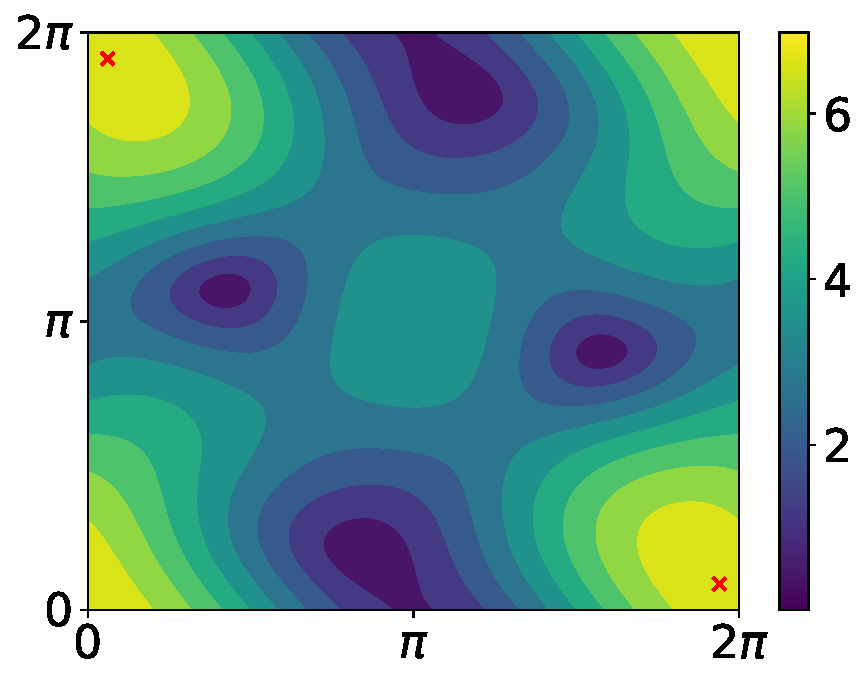
\includegraphics[scale=0.23]{figures/chapter4/contour_poly_200_1_1_3.pdf}\\kernel $1\times3\times3$
  \end{minipage}
  \begin{minipage}{.24\linewidth}
      \centering
      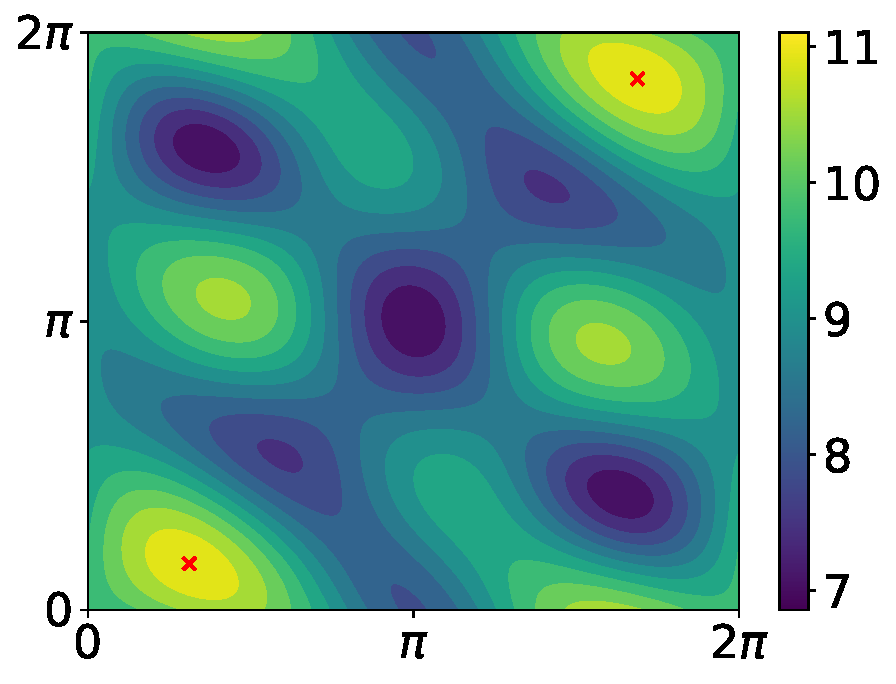
\includegraphics[scale=0.23]{figures/chapter4/contour_poly_200_1_9_3.pdf}\\kernel $9\times3\times3$
  \end{minipage}
  \begin{minipage}{.24\linewidth}
      \centering
      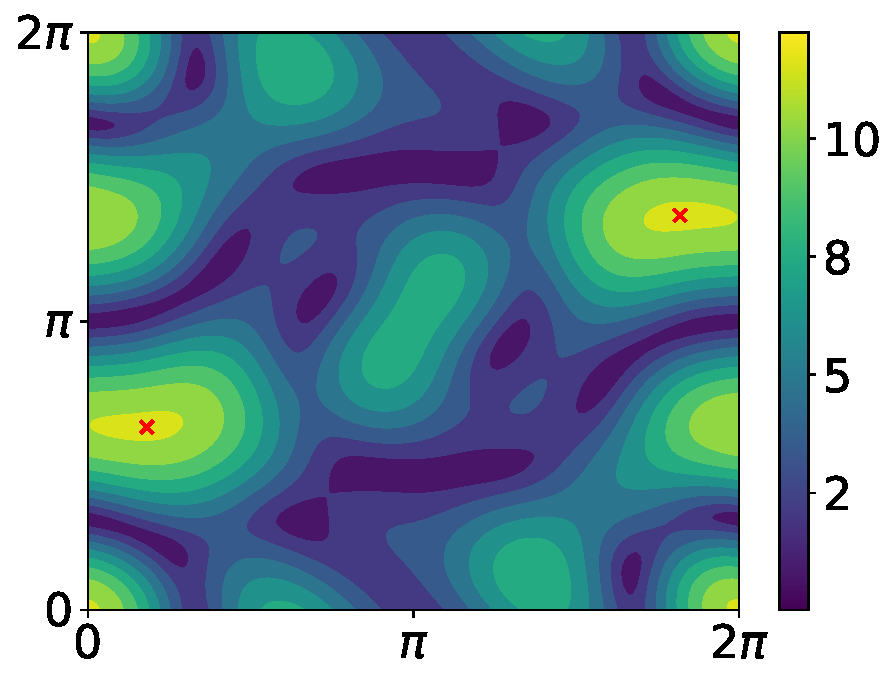
\includegraphics[scale=0.23]{figures/chapter4/contour_poly_200_1_1_5.pdf}\\kernel $1\times5\times5$
  \end{minipage}
  \begin{minipage}{.24\linewidth}
      \centering
      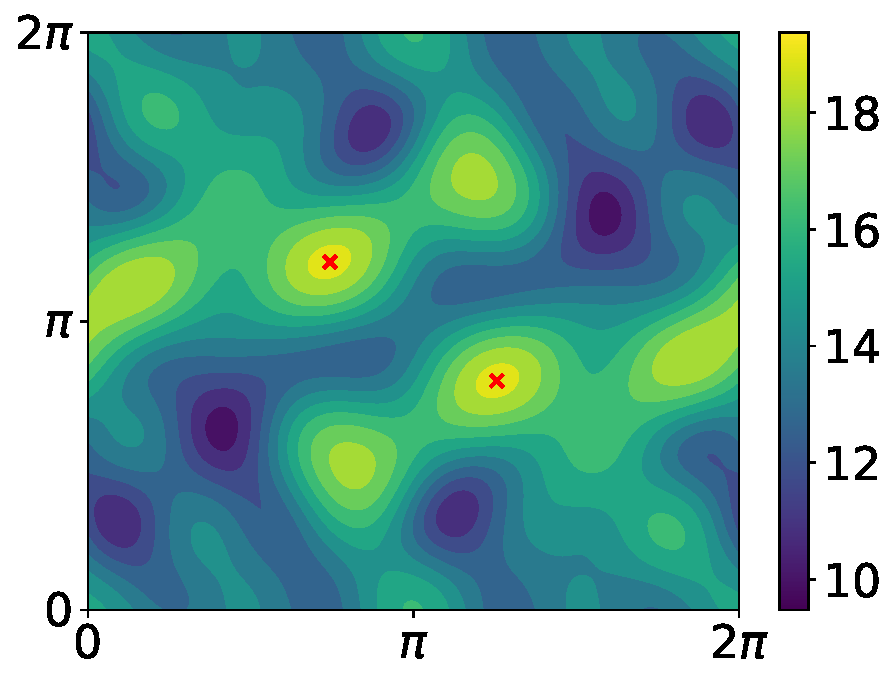
\includegraphics[scale=0.23]{figures/chapter4/contour_poly_200_1_9_5.pdf}\\kernel $9\times5\times5$
  \end{minipage}
  \caption{These figures represent the contour plot of multivariate trigonometric polynomials where the values of the coefficient are the values of a random convolutional kernel. The red dots in the figures represent the maximum modulus of the trigonometric polynomials.}
  \label{figure:contour_plot_trigonometric_polynomials}
\end{figure*}%

\begin{algorithm}
  \caption{PolyGrid Algorithm} \label{algorithm:PolyGrid}
  \begin{algorithmic}[1]
    \Procedure{PolyGrid}{$f, S$}\Comment{polynomial $f$, number of samples $S$}
      \State $\sigma \gets 0$, 
      \State $\omega_1 \gets 0$
      \State $\omega_2 \gets 0$
      \State $\epsilon \gets \frac{2\pi}{S}$
      \For{$i=0$ \textbf{to} $S-1$}
	\For{$j=0$ \textbf{to} $S-1$}
	  \State $\omega_2 \gets \omega_2 + \epsilon$
	  \State $\sigma \gets \max( \sigma, f(\omega_1, \omega_2))$
	\EndFor
      \EndFor
      \State \textbf{return} $\sigma$ \Comment{approximated maximum modulus of $f$}
    \EndProcedure
  \end{algorithmic}
\end{algorithm}

In order to compute $\lipbound$ from Theorem~\ref{theorem:bound_max_sv_convolution}, we have to compute the maximum modulus of several trigonometric polynomials.
However, finding the maximum modulus of a trigonometric polynomial has been known to be NP-Hard~\cite{pfister2018bounding}, and in practice they exhibit low convexity (see Figure~\ref{figure:contour_plot_trigonometric_polynomials}).
We found that for 2-dimensional kernels, a simple grid search algorithm such as PolyGrid (see Algorithm~\ref{algorithm:PolyGrid}), works better than more sophisticated approximation algorithms (\eg ~\citet{green1999calculating,de2009finding}).
This is because the complexity of the computation depends on the degree of the polynomial which is equal to $\lfloor s / 2 \rfloor$ where $s$ is the size of the kernel and is usually small in most practical settings (\eg $s=3$).
Furthermore, the grid search algorithm can be parallelized effectively on CPUs or GPUs and runs within less time than alternatives with lower asymptotic complexity. 

To fix the number of samples $S$ in the grid search, we rely on the work of~\cite{pfister2018bounding}, who has analyzed the quality of the approximation depending on $S$.
Following, this work we first define $\Theta_S$, the set of $S$ equidistant sampling points as follows:
\begin{equation}
  \Theta_S \triangleq \left\{ \omega \mid \omega = k \cdot \frac{2\pi}{S} \mbox{ with }  k = 0,\ldots, S-1 \right\}.
\end{equation}
Then, for a trigonometric polynomial $f: [0, 2\pi]^2 \rightarrow \mathbb{C}$, we have:
\begin{equation}
  \max_{\omega_1, \omega_2 \in [0,2\pi]^2} \left| f(\omega_1, \omega_2) \right| \leq (1 - \alpha)^{-1} \max_{\omega_1', \omega_2' \in \Theta_S^2} \left| f(\omega_1', \omega_2') \right|,
\end{equation}
where $d$ is the degree of the polynomial and $\alpha = 2d / S$.
For a $3\times3$ kernel which gives a trigonometric polynomial of degree 1, we use $S = 10$ which gives $\alpha = 0.2$.
Using this result, we can now compute $\lipbound$ for a convolution operator with $cout$ output channels as per Theorem~\ref{theorem:bound_sv_stacked_dbt}.
 
% The code to for computing $\lipbound$ with NumPy~\cite{numpy} and PyTorch~\cite{paszke2019pytorch} is publicly available.\footnote{\url{https://github.com/MILES-PSL/upper_bound_lipschitz_convolutional_layers}}.


\subsection{Analysis of the tightness of the bound}
\label{section:analysis_tightness_bound}

In this section, we study the tightness of the bound with respect to the dimensions of the doubly-block Toeplitz matrices.
For each $n \in \mathbb{N}$, we define the matrix  $\Mmat^{(n)}$ of size $kn^2 \times n^2$ as follows:
\begin{equation}
  \Mmat^{(n)} \triangleq \textstyle \leftmat \Dmat^{(n)\top}(f_1), \dots, \Dmat^{(n)\top}(f_k) \textstyle \rightmat^\top
\end{equation}
where the matrices $\Dmat^{(n)}(f_i)$ are of size $n^2 \times n^2$. 
To analyze the tightness of the bound, we define the function $\Gamma$, which computes the difference between $\lipbound$ and the maximal singular value of the function $\Mmat^{(n)}$:
\begin{equation} \label{equation:function_convergence}
  \Gamma(n) = \lipbound(\mathbf{k}_{\Mmat^{(n)}}) - \sigma_1(\Mmat^{(n)})
\end{equation}
where $\mathbf{k}_{\Mmat^{(n)}}$ is the  convolution kernel of the convolution defined by the matrix $\Mmat^{(n)}$.

\begin{figure}[ht]
  \centering
  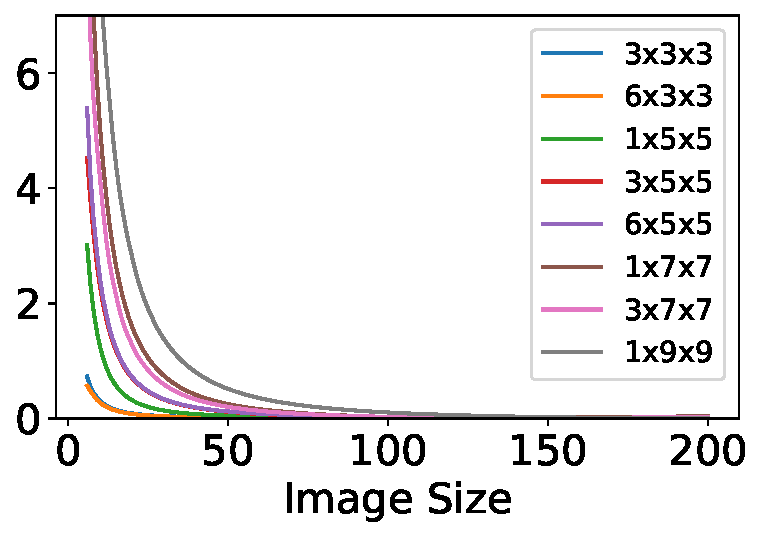
\includegraphics[scale=0.50]{figures/chapter4/convergence_bound.pdf}
  \caption{This graph represents the function $\Gamma(n)$ defined in Section~\ref{section:analysis_tightness_bound} for different kernel size.}
  \label{figure:convergence_bound}
\end{figure}


To compute the exact largest singular value of $\Mmat^{(n)}$ for a specific $n$, we use the Implicitly Restarted Arnoldi Method (IRAM) ~\cite{lehoucq1996deflation} available in SciPy.
The results of this experiment are presented in Figure~\ref{figure:convergence_bound}.
We observe that the difference between the bound and the actual value (approximation gap) quickly decreases as the input size increases.
For an input size of $50$, the approximation gap is as low as $0.012$ using a standard $6\times3\times3$ convolution kernel.
For a larger input size such as ImageNet ($224$), the gap is lower than $4.10^{-4}$.
Therefore $\lipbound$ gives an almost exact value of the maximal singular value of the operator matrix for most realistic settings.

\subsection{Comparison of LipBound with other state-of-the-art approaches} \label{subsection:comparaison_sota}

\begin{table}[ht]
  \centering
  \caption{The following table compares different approaches for computing an approximation of the maximal singular value of a convolutional layer. It shows the ratio between the approximation and the true maximal singular value. The approximation is better for a ratio close to one.}
  {\footnotesize
    \begin{tabular}{lrccrcc}
    \toprule
      &   & \multicolumn{2}{c}{\textbf{1x3x3}} &   & \multicolumn{2}{c}{\textbf{32x3x3}} \\
    \cmidrule{3-4}\cmidrule{6-7}  &   & \textbf{Ratio} & \textbf{Time (ms)} &   & \textbf{Ratio} & \textbf{Time (ms)} \\
    \midrule
    \citeauthor{sedghi2018iclr} &   & $\phantom{.}0.431\pm0.042$ & $1088\pm251$ &   & $\phantom{.}0.666\pm0.123$ & $1729\pm399$ \\
    \citeauthor{singla2019bounding} &   & $\phantom{.}1.293\pm0.126$ & $\phantom{..}1.90\pm0.48$ &   & $\phantom{.}1.441\pm0.188$ & $\phantom{..}1.90\pm0.46$ \\
    \citeauthor{farnia2018generalizable} (10 iter) &   & $\phantom{.}0.973\pm0.006$ & $\phantom{..}4.30\pm0.64$ &   & $\phantom{.}0.972\pm0.004$ & $\phantom{..}4.93\pm0.67$ \\
    \midrule
    \midrule
    \textbf{LipBound (Ours)} &   & $\mathbf{0.992}\pm0.012$ & $\phantom{.}\mathbf{0.49}\pm0.05$ &   & $\mathbf{0.984}\pm0.021$ & $\phantom{.}\mathbf{0.63}\pm0.46$ \\
    \bottomrule
    \end{tabular}%
  }
  \label{table:comparaison}%
\end{table}


In this section we compare our PolyGrid algorithm with the values obtained using alternative approaches.
We consider the 3 alternative techniques by~\citet{sedghi2018iclr,singla2019bounding,farnia2018generalizable} which have been described in Section~\ref{section:ch4-related_work}. 

To compare the different approaches, we extracted 20 kernels from a trained model.
For each kernel we construct the corresponding doubly-block Toeplitz matrix and compute its largest singular value.
Then, we compute the ratio between the approximation obtained with the approach in consideration and the exact singular value obtained by SVD, and average the ratios over the 20 kernels.
Thus good approximations result in approximation ratios that are close to 1.
The results of this experiment are presented in Table~\ref{table:comparaison}.
The comparison has been made on a Tesla V100 GPU. 
The time was computed with the PyTorch CUDA profiler and we warmed up the GPU before starting the timer.

The method introduced by~\citet{sedghi2018iclr} computes an approximation of the singular values of convolutional layers.
We can see in Table~\ref{table:comparaison} that the value is off by an important margin.
This technique is also computationally expensive as it requires computing the SVD of $n^2$ small matrices where $n$ is the size of inputs.
\citet{singla2019bounding} have shown that the singular value of the reshape kernel is a bound on the maximal singular value of the convolution layer.
Their approach is very efficient but the approximation is loose and overestimate the real value.
As said previously, the power method provides a good approximation at the expense of the efficiency.
We use the special Convolutional Power Method from~\citet{farnia2018generalizable} with 10 iterations.
The results show that our proposed technique: PolyGrid algorithm can get the best of both worlds.
It achieves a near perfect accuracy while being very efficient to compute. 

We provide in the supplementary material a benchmark on the efficiency of $\lipbound$ on multiple convolutional architectures. 


%%%%%%%%%%%%%%%%%%%%%%%%%%%%%%%%%%%%%%%%%%%%%%%%%%%%%%%%%%%%%%%%%%%%%%%%%%%%%%%
\section{Application: Lipschitz Regularization for Adversarial Robustness}
\label{section:experiments}
%%%%%%%%%%%%%%%%%%%%%%%%%%%%%%%%%%%%%%%%%%%%%%%%%%%%%%%%%%%%%%%%%%%%%%%%%%%%%%%

\begin{table}[t]
  \centering
  \caption{This table shows the Accuracy under $\ltwo$ and $\linf$ attacks of CIFAR10 dataset. We compare vanilla Adversarial Training with the combination of Lipschitz regularization and Adversarial Training. We also compare the effectiveness of the power method by~\citet{farnia2018generalizable} and $\lipbound$. The parameters $\lambda_2$ from Equation~\ref{equation:objectif_function} is equal to $0.008$ for AT+PM and AT+LipReg. It has been chosen from a grid search among 10 values. The attacks below are computed with 200 iterations. }
    \begin{tabular}{lcccc}
    \toprule
      & \textbf{Accuracy} & \textbf{PGD-$\linf$} & \textbf{C\&W-$\ltwo$ 0.6} & \textbf{C\&W-$\ltwo$ 0.8} \\
    \midrule
    \textbf{Baseline} & $\mathbf{0.953}\pm0.001$ & $\phantom{.}0.000\pm0.000$ & $\phantom{.}0.002\pm0.000$ & $\phantom{.}0.000\pm0.000$ \\
    \textbf{AT} & $\phantom{.}0.864\pm0.001$ & $\phantom{.}0.426\pm0.000$ & $\phantom{.}0.477\pm0.000$ & $\phantom{.}0.334\pm0.000$ \\
    \textbf{AT+PM} & $\phantom{.}0.788\pm0.010$ & $\phantom{.}0.434\pm0.007$ & $\phantom{.}0.521\pm0.005$	 & $\phantom{.}0.419\pm0.003$ \\
    \textbf{AT+LipReg} & $\phantom{.}0.808\pm0.022$ & $\mathbf{0.457}\pm0.002$ & $\mathbf{0.547}\pm0.022$ & $\mathbf{0.438}\pm0.020$ \\
    \bottomrule
    \end{tabular}%
  \label{tab:table_cifar10_robustness}%
\end{table}%

One promising application of Lipschitz regularization is in the area of adversarial robustness.
Empirical techniques to improve robustness against adversarial examples such as Adversarial Training only impact the training data,  and often show poor generalization capabilities~\cite{schmidt2018adversarially}. 
\citet{farnia2018generalizable} have shown that the adversarial generalization error depends on the Lipschitz constant of the network, which suggests that the adversarial test error can be improved by applying Lipschitz regularization in addition to adversarial training. 

In this section, we illustrate the usefulness of LipBound by training a state-of-the-art Wide ResNet architecture~\cite{zagoruyko2016wide} with Lipschitz regularization and adversarial training.
Our regularization scheme is inspired by the one used by~\citet{yoshida2017spectral} but instead of using the power method, we use our \textbf{PloyGrid} algorithm presented in Section~\ref{subsection:computing_max_modulus_trig_polynomial} which efficiently computes an upper bound on the maximal singular value of convolutional layers. 

We introduce the \textbf{AT+LipReg} loss to combine Adversarial Training and our Lipschitz regularization scheme in which layers with a large Lipschitz constant are penalized.
We consider a neural network $\mathcal N_\theta : \mathcal X \rightarrow \mathcal Y$ with $\ell$ layers $\phi^{(1)}_{\theta_1}, \ldots, \phi^{(\ell)}_{\theta_\ell}$ where $\theta^{(1)}, \ldots, \theta^{(\ell -1)}$ are the kernels of the first $\ell - 1$ convolutional layers and $\theta_\ell$ is the weight matrix of the last fully-connected  layer $\phi^{(\ell)}_{\theta_\ell}$.
Given a distribution $\mathcal D$ over $\mathcal X \times \mathcal Y$, we can train the parameters $\theta$ of the network by minimizing the AT+LipReg loss as follows:
\begin{equation} \label{equation:objectif_function}
    \min_{\theta} \mathbb E_{x,y \sim \mathcal D} \left[ \max_{\norm{\tau}_\infty \leq \epsilon} \mathcal{L}(\mathcal{N}_\theta(x + \tau), y)  + \lambda_1 \sum_{i=1}^\ell {\textstyle \norm{\theta_i}_\text{F}} + \lambda_2 \sum_{i=1}^{\ell-1} \log\left( \lipbound\left(\theta_i\right)\right) \right]
\end{equation}
where $\mathcal L$ is the cross-entropy loss function, and $\lambda_1$, $\lambda_2$ are two user-defined hyper-parameters.
Note that regularizing the sum of logs is equivalent to regularizing the product of all the $\lipbound$ which is an upper bound on the global Lipschitz constant.
In practice, we also include the upper bound on the Lipschitz of the batch normalization because we can compute it very efficiently (see C.4.1 of~\citet{tsuzuku2018lipschitz}) but we omit the last fully connected layer. 

\begin{figure}[ht]
   \centering
   \begin{subfigure}[b]{0.49\textwidth}
       \centering
       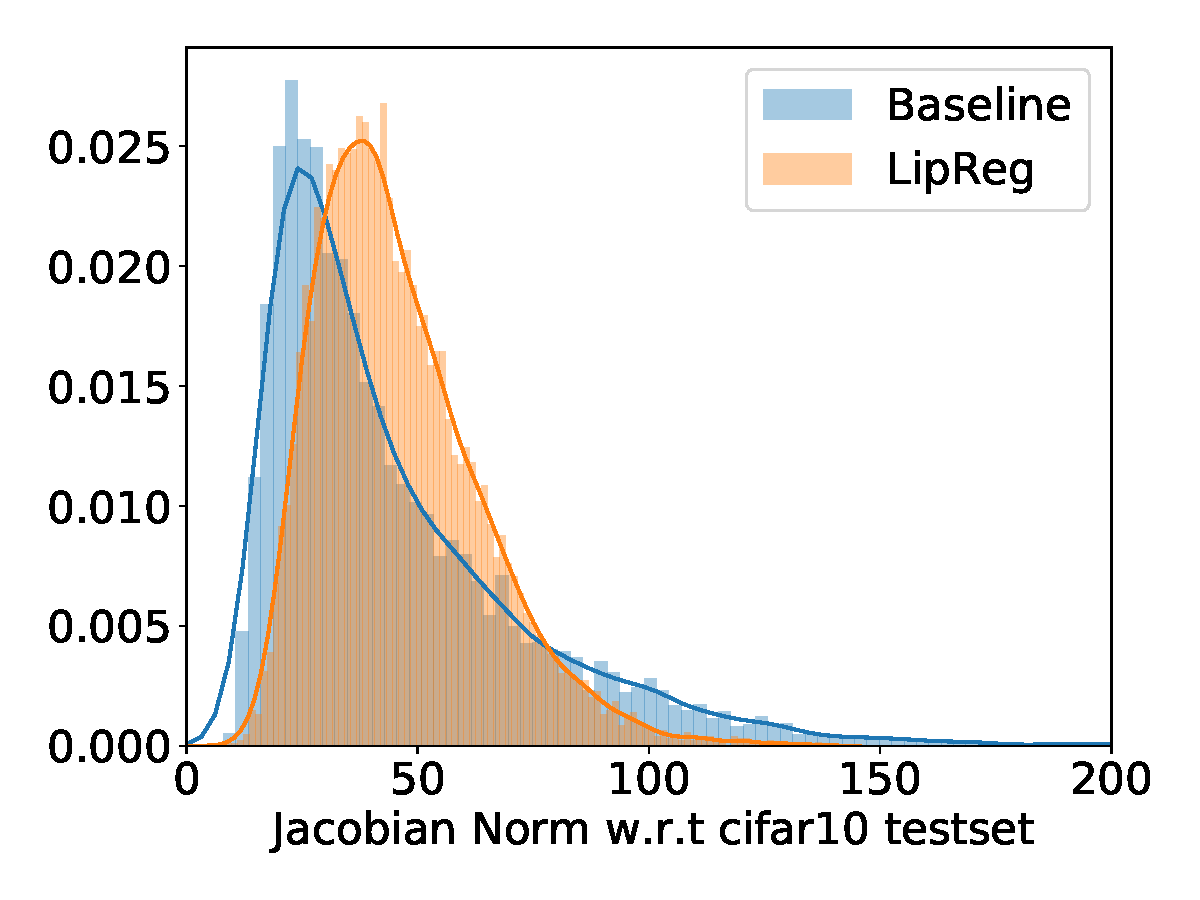
\includegraphics[width=\textwidth]{figures/chapter4/jacobian_distribution_v1.pdf}\\(a)
   \end{subfigure}
   \hfill
   \begin{subfigure}[b]{0.49\textwidth}
       \centering
       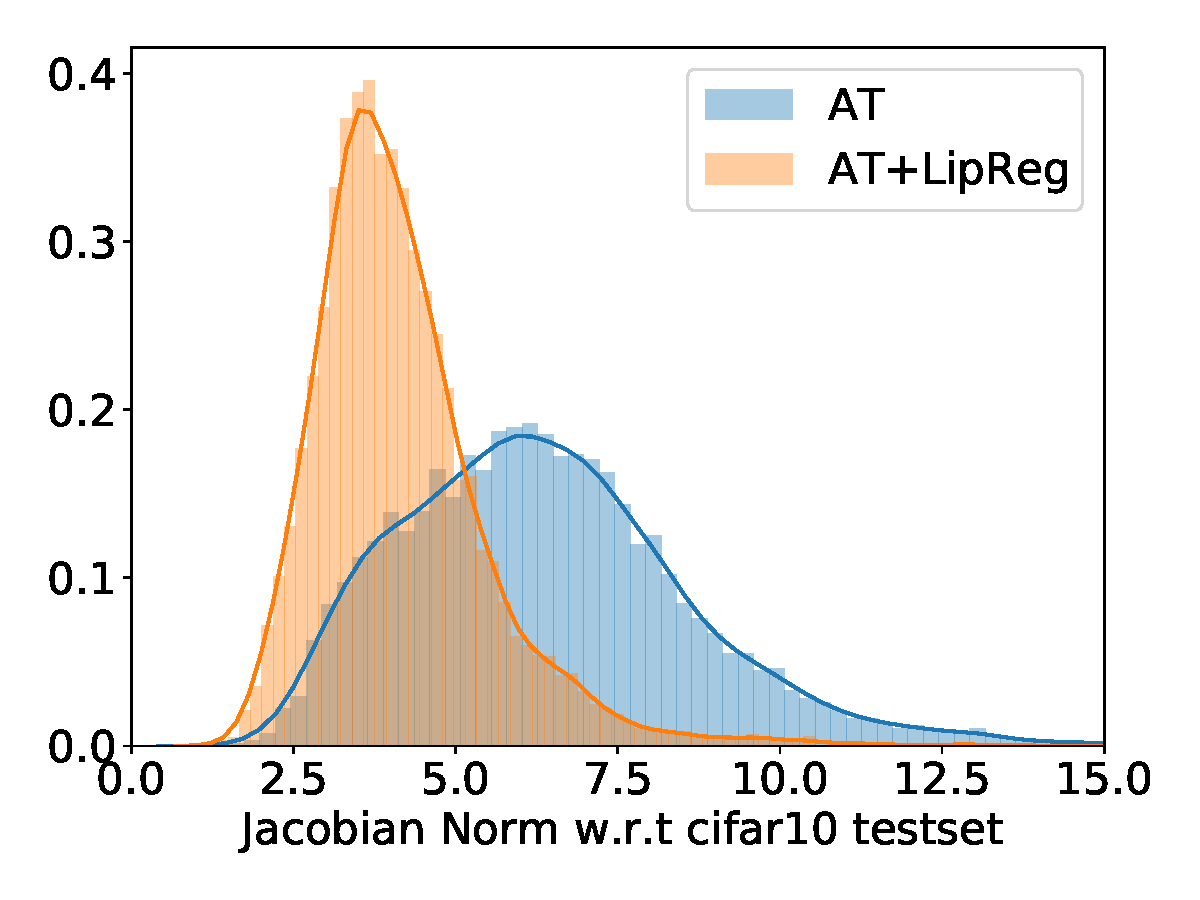
\includegraphics[width=\textwidth]{figures/chapter4/jacobian_distribution_v2.pdf}\\(b)
   \end{subfigure}
   \caption{These figures show the distribution of the norm of the Jacobian matrix w.r.t the CIFAR10 test set from a Wide Resnet trained with different schemes. Although Lipschitz regularization is not a Jacobian regularization, we can observe a clear shift in the distribution. This suggests that our method does not only work layer-wise, but also at the level of the entire network.}
   \label{figure:jacobian_distribution}
\end{figure}


\begin{figure}[ht]
   \centering
   \begin{subfigure}[b]{0.49\textwidth}
       \centering
       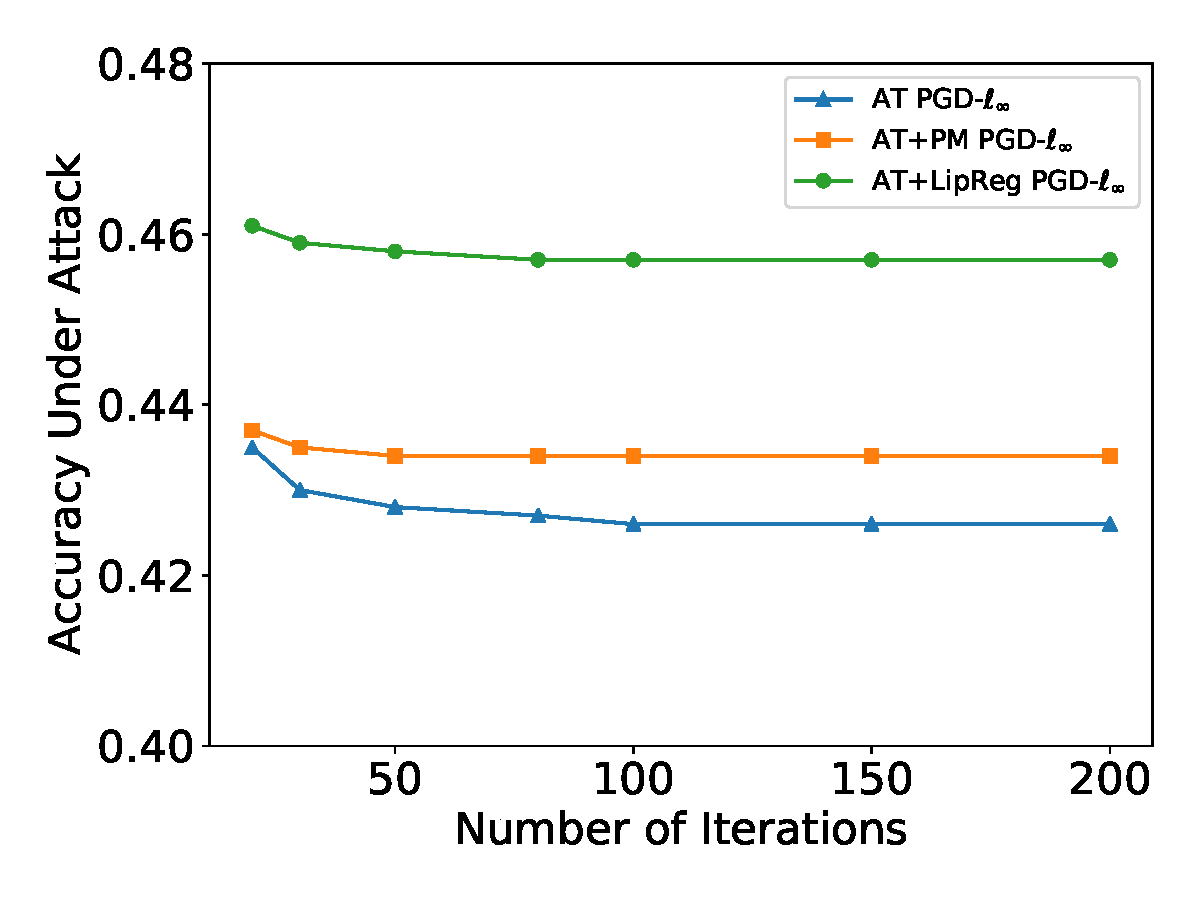
\includegraphics[width=\textwidth]{figures/chapter4/attacks_iter_pgd.pdf}\\(a)
   \end{subfigure}
   \hfill
   \begin{subfigure}[b]{0.49\textwidth}
       \centering
       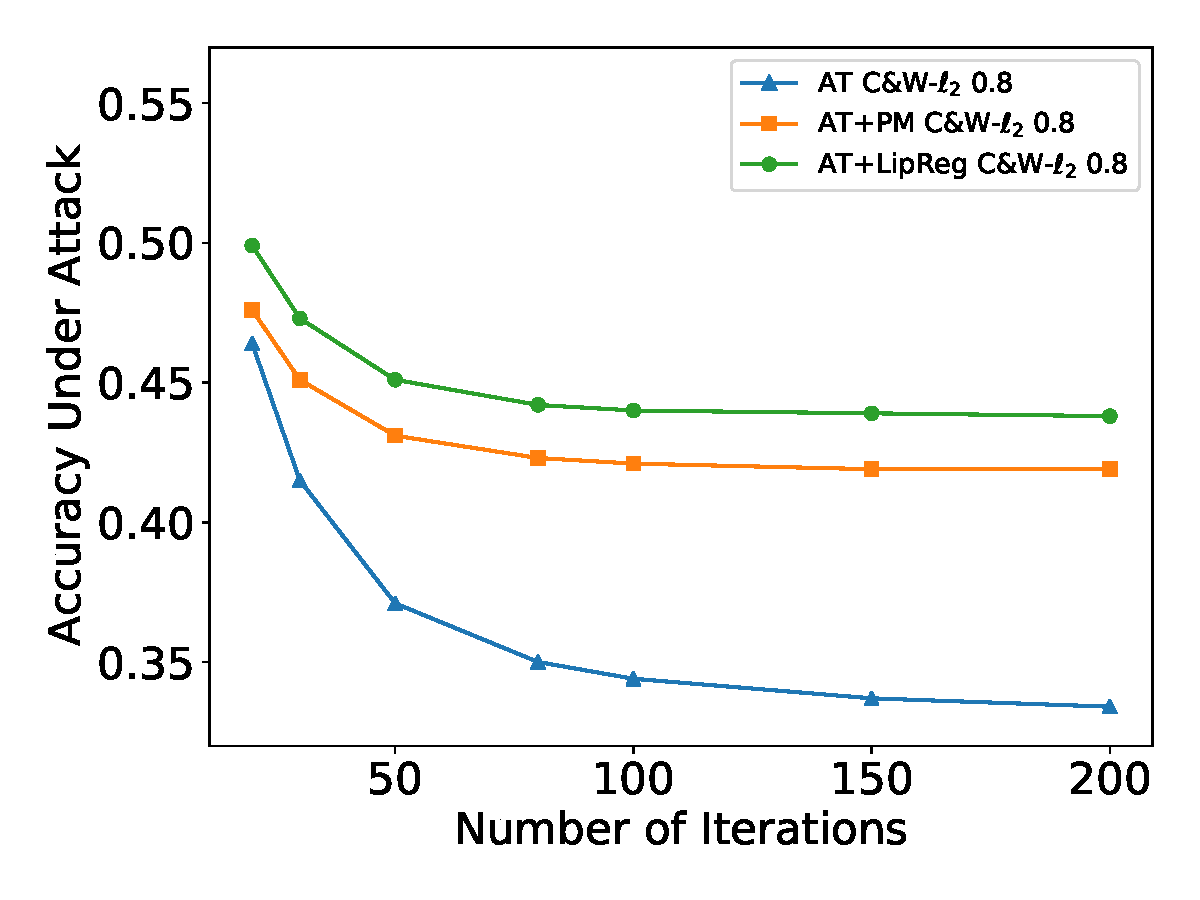
\includegraphics[width=\textwidth]{figures/chapter4/attacks_iter_cw.pdf}\\(b)
   \end{subfigure}
   \caption{These figures show the Accuracy under attack on CIFAR10 test set with PGD-$\linf$ and C\&W-$\ltwo$ attacks for several classifiers trained with Adversarial Training given the number of iterations.}
   \label{figure:attacks_iter}
\end{figure}


% \begin{figure*}[htb]
%   \centering
%   \begin{minipage}{.24\linewidth}
%     \centering
%     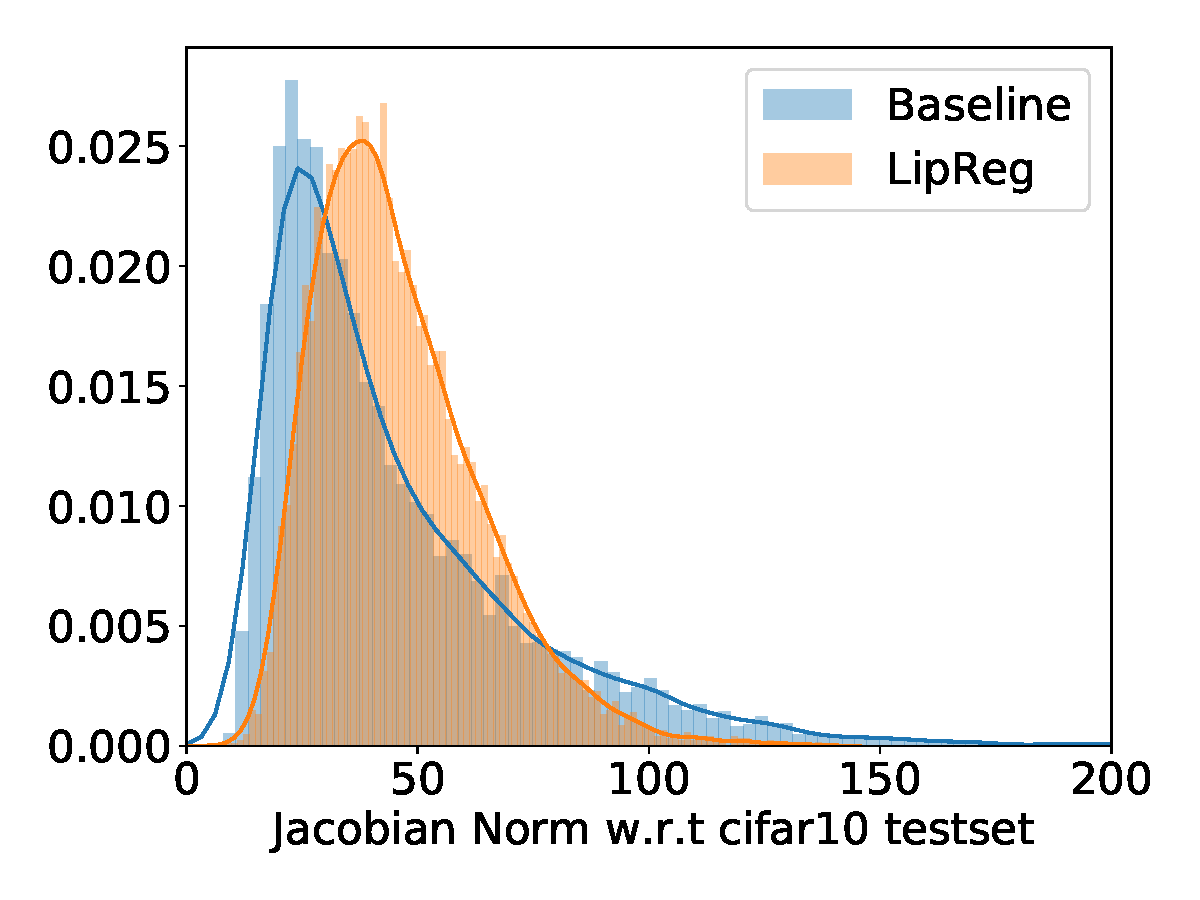
\includegraphics[scale=0.16]{figures/chapter4/jacobian_distribution_v1.pdf}\\{(a)}
%   \end{minipage}
%   \hfill
%   \begin{minipage}{.24\linewidth}
%     \centering
%     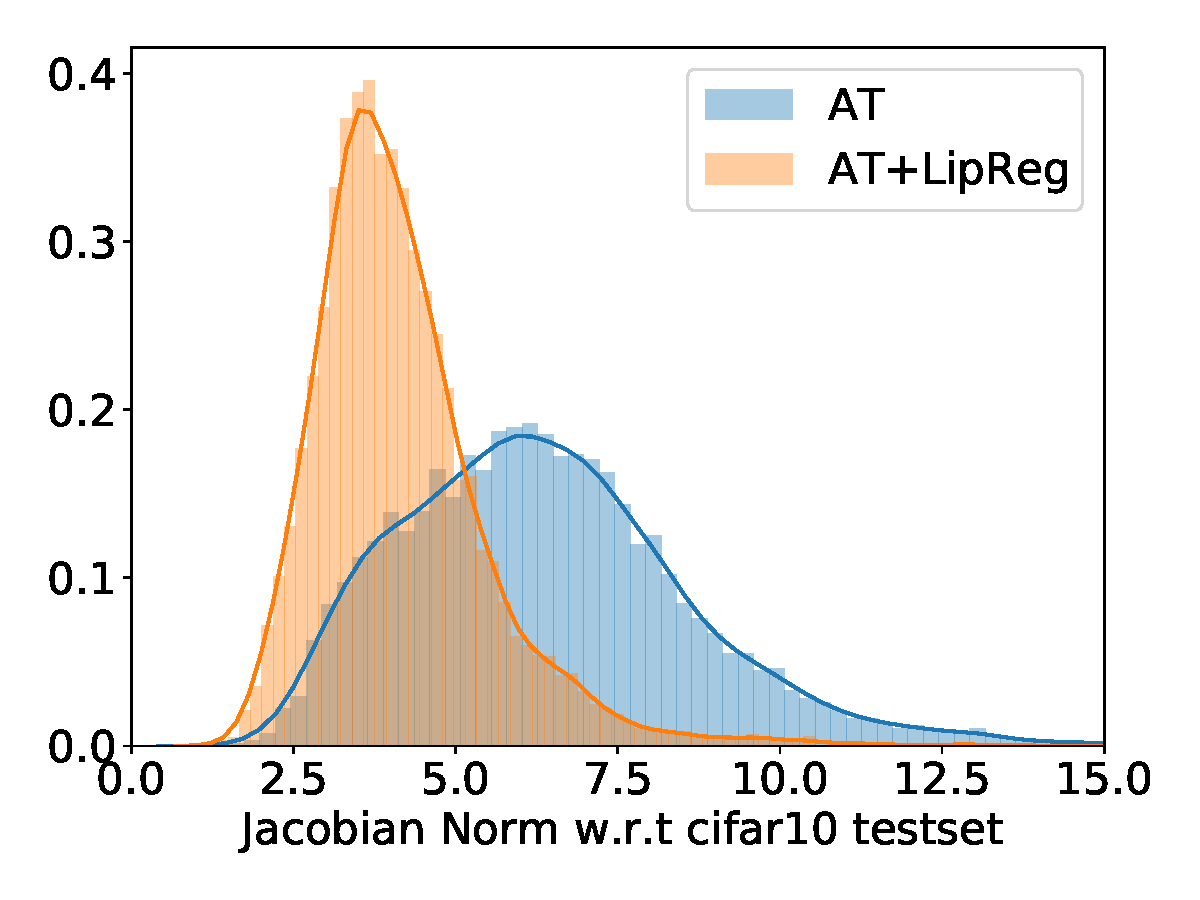
\includegraphics[scale=0.16]{figures/chapter4/jacobian_distribution_v2.pdf}\\{(b)}
%   \end{minipage}
%   \hfill
%   \begin{minipage}{.24\linewidth}
%     \centering
%     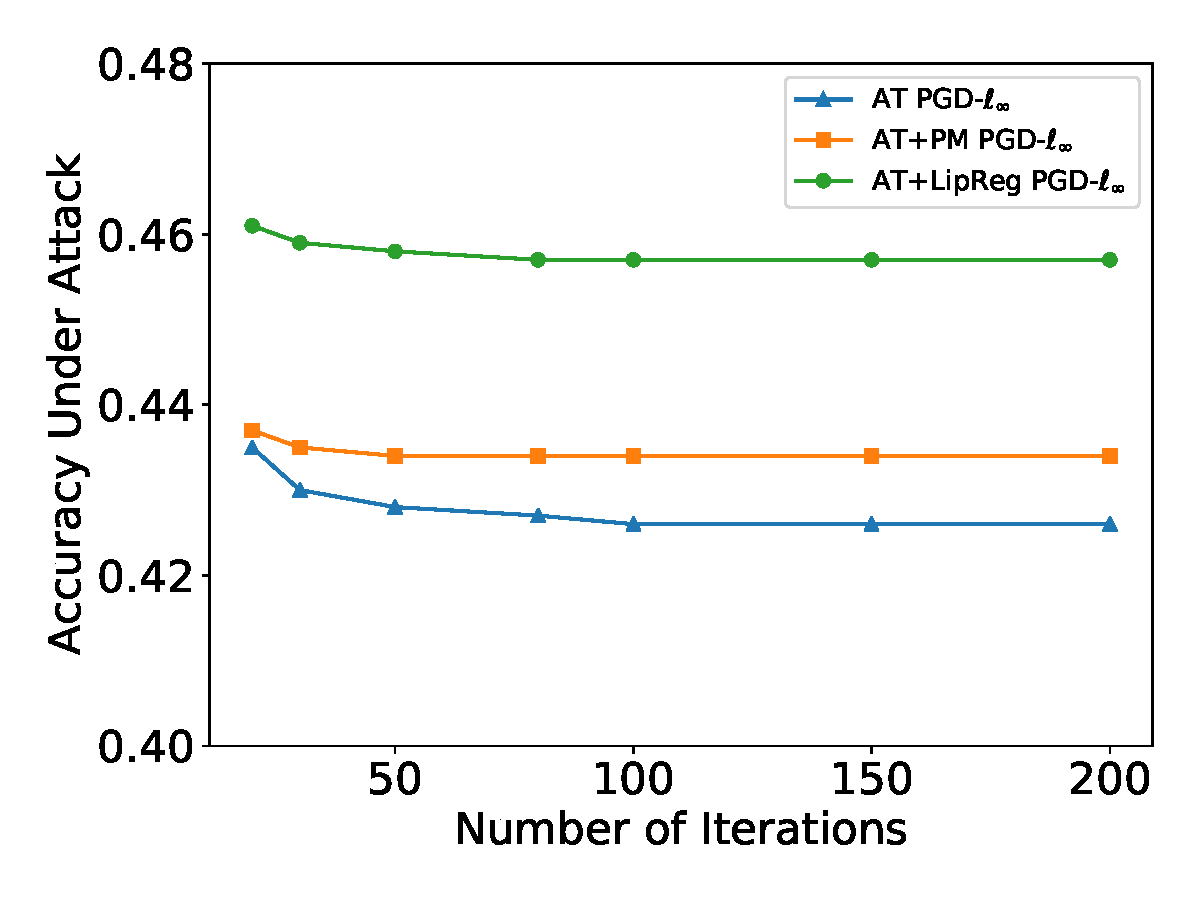
\includegraphics[scale=0.16]{figures/chapter4/attacks_iter_pgd.pdf}\\{(c)}
%   \end{minipage}
%   \hfill
%   \begin{minipage}{.24\linewidth}
%     \centering
%     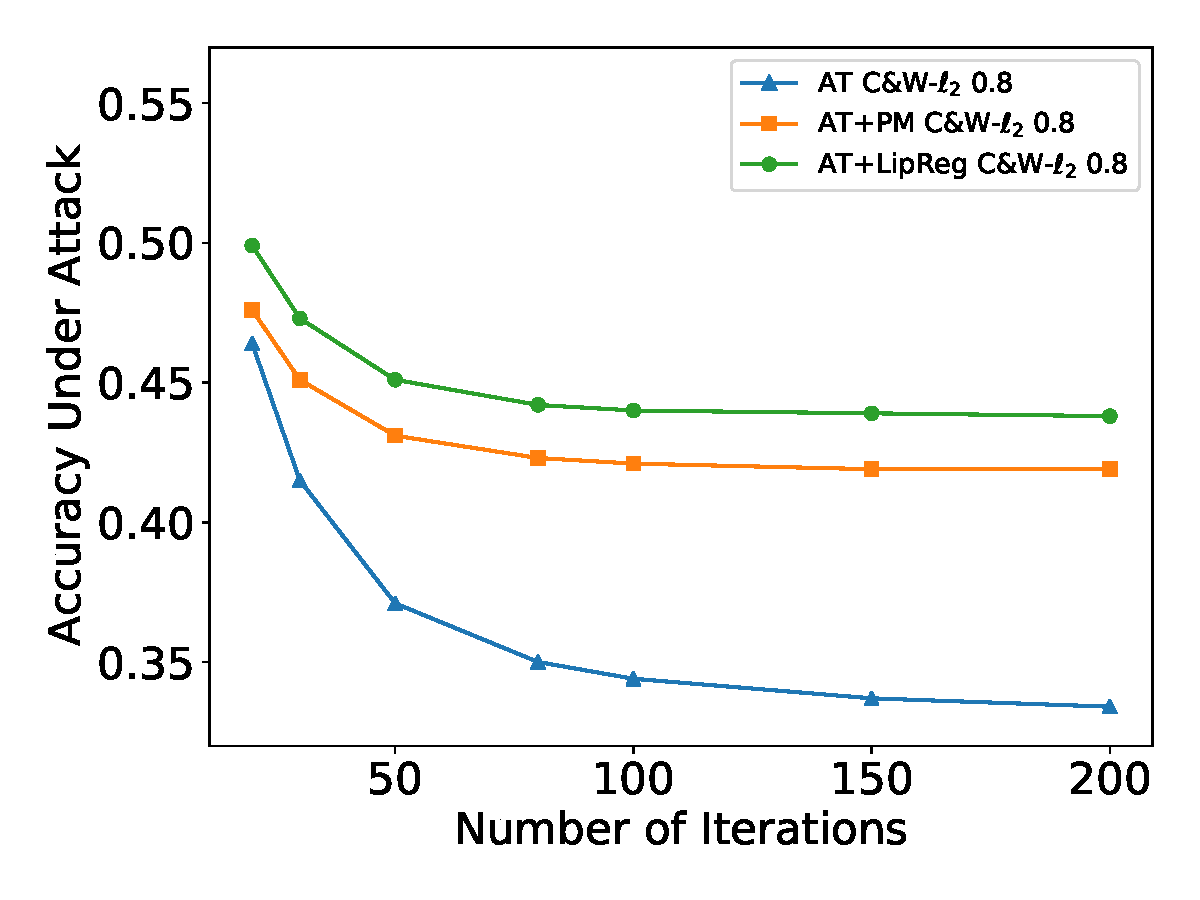
\includegraphics[scale=0.16]{figures/chapter4/attacks_iter_cw.pdf}\\{(d)}
%   \end{minipage}
%   \caption{Figures (a) and (b) show the distribution of the norm of the Jacobian matrix w.r.t the CIFAR10 test set from a Wide Resnet trained with different schemes. Although Lipschitz regularization is not a Jacobian regularization, we can observe a clear shift in the distribution. This suggests that our method does not only work layer-wise, but also at the level of the entire network. Figures (c) and (d) show the Accuracy under attack on CIFAR10 test set with PGD-$\linf$ and C\&W-$\ltwo$ attacks for several classifiers trained with Adversarial Training given the number of iterations.}
%   \label{figure:dist_jacobian_attacks_iter}
% \end{figure*}%


In this section, we compare the robustness of Adversarial Training~\cite{goodfellow2014explaining, madry2018towards} against the combination of Adversarial Training and Lipschitz regularization.
To regularize the Lipschitz constant of the network, we use the objective function defined in Equation~\ref{equation:objectif_function}.
We train Lipschitz regularized neural network with LipBound (Theorem~\ref{theorem:bound_max_sv_convolution}) implemented with PolyGrid (Algorithm~\ref{algorithm:PolyGrid}) (AT+LipBound) with $S = 10$ or with the specific power method for convolutions introduced by~\citet{farnia2018generalizable} with 10 iterations (AT+PM). 

Table~\ref{tab:table_cifar10_robustness} shows the gain in robustness against strong adversarial attacks.
We can observe that both AT+LipBound and AT+PM offer a better defense against adversarial attacks and that AT+LipBound offers a further improvement over the Power Method.
The Figure~\ref{figure:attacks_iter} (b) shows the Accuracy under attack with different number of iterations. 

Finally, we also conducted an experiment to study the impact of the regularization on the gradients of the whole network by measuring the norm of the Jacobian matrix, averaged over the inputs from the test set.
The results of this experiment are presented in Figure~\ref{figure:jacobian_distribution} (a) and show more concentrated gradients with Lipschitz regularization, which is the expected effect.
This suggests that our method does not only work layer-wise, but also at the level of the entire network.
A second experiment, using Adversarial Training, presented in Figure~\ref{figure:jacobian_distribution} (b) demonstrates that the effect is even stronger when the two techniques are combined together.
This corroborates the work by~\cite{farnia2018generalizable}.
It also demonstrates that Lipschitz regularization and Adversarial Training (or other Jacobian regularization techniques) are complementary.
Hence they offer an increased robustness to adversarial attacks as demonstrated above.

\paragraph{Experimental Settings}
We use the Wide ResNet architecture introduced by~\citet{zagoruyko2016wide} to train our classifiers (for details of the hyper-parameters used, see the supplementary material).
For Adversarial Training ~\cite{madry2018towards}, we use Projected Gradient Descent with an $\epsilon = 8/255 (\approx 0.031)$, a step size of $\textstyle \frac{\epsilon}{5} (\approx 0.0062)$ and 10 iterations, we use a random initialization but run the attack only once.
To evaluate the robustness of our classifiers, we rigorously followed the experimental protocol proposed by~\citet{tramer2020adaptive} and~\citet{carlini2019evaluating}.
More precisely, as an $\linf$ attack, we use PGD with the same parameters ($\epsilon = 8/255$, a step size of $\textstyle \frac{\epsilon}{5}$) but we increase the number of iterations up to 200 with 10 restarts.
For each image, we select the perturbation that maximizes the loss among all the iterations and the 10 restarts.
As $\ltwo$ attacks, we use a bounded version of the~\cite{carlini2017towards} attack.
We choose $0.6$ and $0.8$ as bounds for the $\ltwo$ perturbation. Note that the $\ltwo$ ball with a radius of $0.8$ has approximately the same volume as the $\linf$ ball with a radius of $0.031$ for the dimensionality of CIFAR10. 


\subsection{Results on CIFAR100 dataset \& Hyper-parameters}

\begin{table}[htb]
  \centering
  \caption{This table shows the Accuracy under $\ltwo$ and $\linf$ attacks of CIFAR100 dataset. We compare Adversarial Training with the combination of Lipschitz regularization and Adversarial Training \cite{madry2018towards}. The $\lambda_2$ parameters which control the Lipschitz regularization is $0.008$, it has been chosen among a grid search of 10 values. The attacks below are computed with 200 iterations.}
    \begin{tabular}{lcccc}
    \toprule
      & \textbf{Accuracy} & \textbf{PGD-$\linf$} & \textbf{C\&W-$\ltwo$ 0.6} & \textbf{C\&W-$\ltwo$ 0.8} \\
    \midrule
    \textbf{Baseline} & $\mathbf{0.792}\pm0.000$ & $\phantom{.}0.000\pm0.000$ & $\phantom{.}0.001\pm0.000$ & $\phantom{.}0.000\pm0.000$ \\
    \textbf{AT} & \phantom{.}$0.591\pm0.000$ & $\phantom{.}0.199\pm0.000$ & $\phantom{.}0.263\pm0.000$ & $\phantom{.}0.183\pm0.000$ \\
    \textbf{AT+LipReg} & \phantom{.}$0.552\pm0.019$ & $\mathbf{0.215}\pm0.004$ & $\mathbf{0.294}\pm0.010$ & $\mathbf{0.226}\pm0.008$ \\
    \bottomrule
    \end{tabular}%
  \label{tab:results_cifar100}%
\end{table}%


\paragraph{Hyper-parameters used for training classifiers on CIFAR10 \& CIFAR100 dataset}
For all our experiments, we use the Wide Resnet architecture \cite{zagoruyko2016wide} with 28 layers and a width factor of 10. We train our networks for 200 epochs with a batch size of $200$. We use Stochastic Gradient Descent with a momentum of $0.9$, an initial learning rate of $0.1$ with exponential decay of 0.1 (MultiStepLR gamma = 0.1) after the epochs $60$, $120$ and $160$. 

\subsection{Results on ImageNet dataset \& Hyper-parameters}

\begin{table}[htb]
  \centering
  \caption{This table shows the accuracy and accuracy under attack of ImageNet dataset with different training schemes. We compare Adversarial Training with the combination of Lipschitz regularization and Adversarial Training \cite{madry2018towards}. }
    {\footnotesize
    \begin{tabular}{lccccccccc}
    \toprule
      & \multicolumn{1}{c}{\multirow{2}[4]{*}{$\lambda_2$}} & \multicolumn{1}{c}{\multirow{2}[4]{*}{\textbf{Natural}}} &   & \multicolumn{2}{c}{\textbf{PGD-}$\linf$} &   & \multicolumn{3}{c}{\textbf{C\&W-}$\ltwo$} \\
\cmidrule{5-6}\cmidrule{8-10}      &   &   &   & \multicolumn{1}{c}{0.02} & \multicolumn{1}{c}{0.031} &   & \multicolumn{1}{c}{1.00} & \multicolumn{1}{c}{2.00} & \multicolumn{1}{c}{3.00} \\
    \midrule
    \textbf{AT} & \multicolumn{1}{c}{-} & 0.509 &   & 0.251 & 0.118 &   & 0.307 & 0.168 & 0.099 \\
    \textbf{AT+LipReg} & 0.0006 & \textbf{0.515} &   & \textbf{0.255} & \textbf{0.121} &   & \textbf{0.316} & \textbf{0.177} & \textbf{0.105} \\
    \textbf{AT+LipReg} & 0.0010 & \textbf{0.519} &   & \textbf{0.259} & \textbf{0.123} &   & \textbf{0.338} & \textbf{0.204} & \textbf{0.129} \\
    \bottomrule
    \end{tabular}%
    }
\end{table}%


\paragraph{Hyper-parameters used for training and attacking classifiers on ImageNet dataset}

For all our experiments, we use the Resnet-101 architecture \cite{he2016deep}. We have used Stochastic Gradient Descent with a momentum of $0.9$, a weight decay of $0.0001$, label smoothing of $0.1$, an initial learning rate of $0.1$ with exponential decay of $0.1$ (MultiStepLR gamma = $0.1$) after the epochs $30$ and $60$. We have used Exponential Moving Average over the weights with a decay of $0.999$. We have trained our networks for 80 epochs with a batch size of $4096$. For Adversarial Training, we have used PGD with 5 iterations, $\epsilon = 8/255 (\approx 0.031)$ and a step size of $\frac{\epsilon}{5} (\approx 0.0062)$. 

To evaluate the robustness of our classifiers in ImageNet, we have used an $\linf$ and an $\ltwo$ attacks. More precisely, as an $\linf$ attack, we use PGD with an epsilon of 0.02 and 0.031, a step size of $\textstyle \frac{\epsilon}{5}$) but we increase the number of iterations to 30 with 5 restarts. For each image, we select the perturbation that maximizes the loss among all the iterations and the 10 restarts. As $\ltwo$ attacks, we use a bounded version of the~\cite{carlini2017towards} attack. We have used $1$, $2$ and $3$ as bounds for the $\ltwo$ perturbation. 


%%%%%%%%%%%%%%%%%%%%%%%%%%%%%%%%%%%%%%%%%%%%%%%%%%%%%%%%%%%%%%%%%%%%%%%%%%%%%%%
\section{Conclusion}
\label{section:ch4-conclusion}
%%%%%%%%%%%%%%%%%%%%%%%%%%%%%%%%%%%%%%%%%%%%%%%%%%%%%%%%%%%%%%%%%%%%%%%%%%%%%%%

In this chapter, we introduced a new bound on the Lipschitz constant of convolutional layers that is both accurate and efficient to compute.
We used this bound to regularize the Lipschitz constant of neural networks and demonstrated its computational efficiency in training large neural networks with a regularized Lipschitz constant.
As an illustrative example, we   combined our bound with adversarial training, and showed that this increases the robustness of the trained networks to  adversarial attacks.
The scope of our results goes beyond this application and can be used  in a wide variety of settings, for example, to stabilize Generative Adversarial Networks, or improve generalization capabilities of classifiers, to mention a few.
Our future work will focus on investigating these fields. 



% \section{Notations}
% Below are the notations we will use for the theorems and proofs. 
% \begin{itemize}
% \itemsep0em 
%     \item Let $\ci = \sqrt{-1}$.
%     \item We denote $\sigma_1(\Amat) = \sigma_{max}(\Amat)$ the maximum singular value of the matrix $\Amat$. 
%     \item We denote $\lambda_1(\Amat) = \lambda_{max}(\Amat)$ the maximum eigenvalue of the Hermitian matrix $\Amat$. 
%     \item For any function $f: \mathcal{X} \rightarrow \mathbb{C}$, we denote $f^*$ the conjugate function of $f$.
%     \item Let $\Amat$ be a $n \times n$ symmetric real matrix, we say that 
%     \begin{itemize}
%         \item[] $\Amat$ is positive definite, and we note $\Amat > 0$ if $\mathbf{x}^{\top} \Amat \mathbf{x} > 0$ for all non-zero $\mathbf{x}$ in $\mathbb{R}^{n}$.
%         \item[] $\Amat$ is positive semi-definite, and we note $\Amat \geq 0$ if $\mathbf{x}^{\top} \Amat \mathbf{x} \geq 0$ for all non-zero $\mathbf{x}$ in $\mathbb{R}^{n}$.
%     \end{itemize}
%     \item Let $N = \{ -n+1, \dots, n-1 \}$ and $M = \{ -m+1, \dots, m-1 \}$
% \end{itemize}


% \section{Discussion on the Convolution Operation}



%
% \section{Additional Results and Discussions on the Experiments}
%
%
%
% \subsection{Additional Results and Discussion of Section~\ref{subsection:comparaison_sota}}
%
%
% \begin{table}[htb]
%   \centering
%   \caption{This table shows the efficiency of LipBound computation vs the Power Method with 10 iterations on the full networks.}
%   {\footnotesize
%     \begin{tabular}{llllr}
%     \toprule
%       &   & \multicolumn{1}{c}{\textbf{LipBound (ms)}} & \multicolumn{1}{c}{\textbf{Power Method (ms)}} & \textbf{Ratio} \\
%     \midrule
%      \cite{krizhevsky2012imagenet} & \textbf{AlexNet} & \phantom{....}$4.75\pm1.1$ & \phantom{....}$38.75\pm2.52$ & \textbf{8.14 }\\
%     \midrule
%     \multirow{5}[2]{*}{\cite{he2016deep}} & \textbf{ResNet 18} & \phantom{..}$29.88\pm1.73$ & \phantom{..}$148.35\pm14.92$ & \textbf{4.96 }\\
%       & \textbf{ResNet 34} & \phantom{..}$54.73\pm3.62$ & \phantom{..}$266.85\pm25.35$ & \textbf{4.87 }\\
%       & \textbf{ResNet 50} & \phantom{..}$60.77\pm4.62$ & \phantom{..}$467.61\pm36.52$ & \textbf{7.69 }\\
%       & \textbf{ResNet 101} & $102.72\pm11.53$ & \phantom{..}$817.06\pm102.87$ & \textbf{7.95 }\\
%       & \textbf{ResNet 152} & $158.80\pm20.84$ & $1373.57\pm164.37$ & \textbf{8.64} \\
%     \midrule
%     \multirow{4}[2]{*}{\cite{huang2017densely}} & \textbf{DenseNet 121} & $125.55\pm14.59$ & \phantom{..}$937.35\pm11.52$ & \textbf{7.46 }\\
%       & \textbf{DenseNet 161} & $176.11\pm19.13$ & $1292.61\pm30.5$ & \textbf{7.33} \\
%       & \textbf{DenseNet 169} & $188.03\pm19.74$ & $1372.62\pm21.16$ & \textbf{7.29} \\
%       & \textbf{DenseNet 201} & $281.13\pm23.41$ & $1930.19\pm170.79$ & \textbf{6.86 }\\
%     \midrule
%     \multirow{4}[2]{*}{\cite{simonyan2014very}} & \textbf{VGG 11} & \phantom{..}$13.73\pm1.19$ & \phantom{....}$81.78\pm4.45$ & \textbf{5.95 }\\
%       & \textbf{VGG 13} & \phantom{..}$14.96\pm1.99$ & \phantom{..}$102.04\pm4.2$ & \textbf{6.82 }\\
%       & \textbf{VGG 16} & \phantom{..}$21.92\pm1.94$ & \phantom{..}$132.29\pm5.99$ & \textbf{6.03 }\\
%       & \textbf{VGG 19} & \phantom{..}$29.05\pm0.66$ & \phantom{..}$162.28\pm4.87$ & \textbf{5.58 }\\
%     \midrule
%     \cite{zagoruyko2016wide} & \textbf{WideResnet 50-2} & $113.28\pm45.44$ & \phantom{..}$468.74\pm6.54$ & \textbf{4.13 }\\
%     \midrule
%     \multirow{2}[2]{*}{\cite{iandola2016squeezenet}} & \textbf{SqueezeNet 1-0} & \phantom{..}$18.44\pm5.93$ & \phantom{....}$222.4\pm25.49$ & \textbf{12.05} \\
%       & \textbf{SqueezeNet 1-1} & \phantom{..}$18.26\pm6.65$ & \phantom{....}$209.8\pm3.59$ & \textbf{11.48} \\
%     \bottomrule
%     \end{tabular}%
%     }
%   \label{tab:efficiency_lipbound_full_model}%
% \end{table}%
%
% The comparison of Table~\ref{table:comparaison} of Section~\ref{subsection:comparaison_sota} of the main paper has been made with the following code provided by the authors: 
% \begin{itemize}
%     \item \makebox[3.2cm]{\cite{sedghi2018iclr}\hfill} \url{https://github.com/brain-research/conv-sv}
%     \item \makebox[3.2cm]{\cite{singla2019bounding}\hfill} \url{https://github.com/singlasahil14/CONV-SV}
%     \item \makebox[3.2cm]{\cite{farnia2018generalizable}\hfill} \url{https://github.com/jessemzhang/dl_spectral_normalization}
% \end{itemize}
% We translated the code of \cite{sedghi2018iclr} from TensorFlow to PyTorch in order to use the PyTorch CUDA Profiler.
%
% We extended the experiments presented in Table~\ref{table:comparaison} of Section~\ref{subsection:comparaison_sota} with Table~\ref{tab:efficiency_lipbound_full_model}.
% This table shows the efficiency of LipBound computation vs the Power Method with 10 iterations on the full network (\ie on all the convolutions of each network).
% The Ratio represents the \emph{speed gain} between our proposed method and the Power Method. 
%
% % \subsection{Additional Results of Section~\ref{section:experiments} \& Hyper-parameters}
%
%
% \subsection{The Effect of Lipschitz Regularization on the Maximal Singular Value of Convolution Layer}
%
% \begin{figure*}[htb]
%     \centering
%     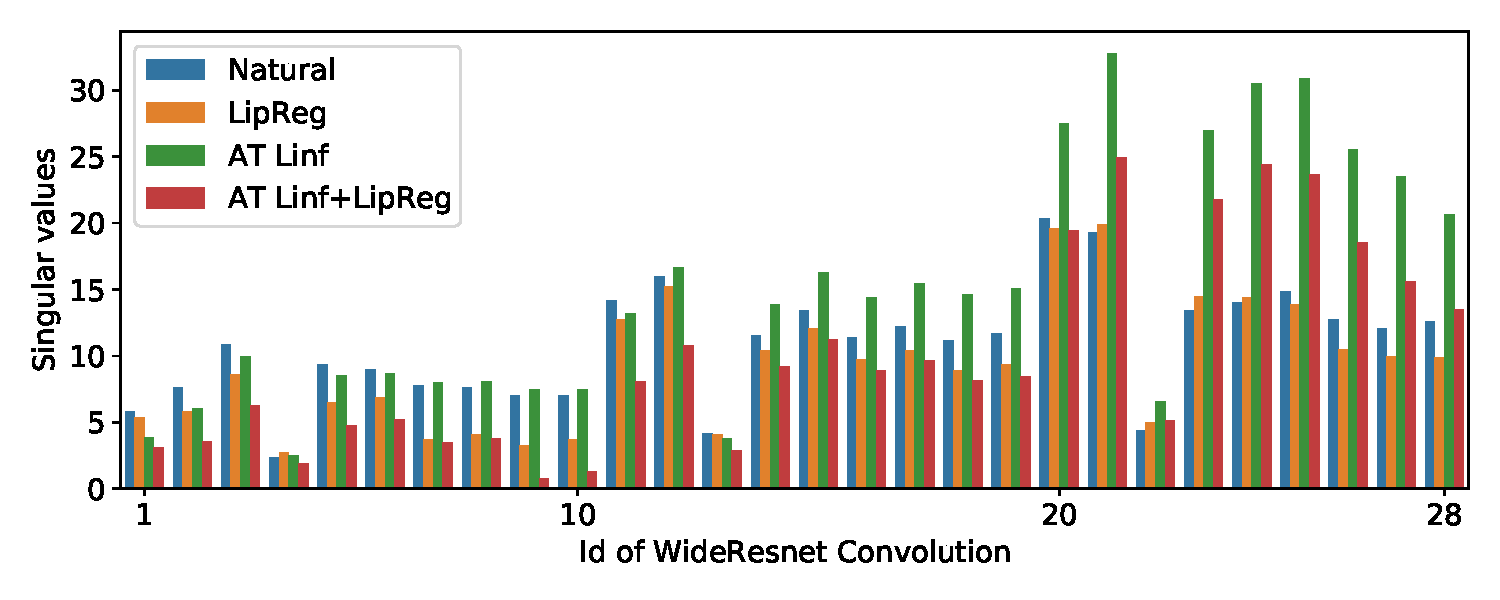
\includegraphics[scale=0.55]{figures/chapter4/singular_values.pdf}
%     \caption{This figure shows the maximal singular values of each convolution of a trained Wide ResNet on CIFAR10 dataset given different training scheme. The id 1 and 28 correspond to the first layer and last layer of the network.}
%     \label{figure:singular_values}
% \end{figure*}%
%
% Figure~\ref{figure:singular_values} shows the maximal singular values of each convolution of a trained Wide ResNet on CIFAR10 dataset given different training scheme. We can observe a small but clear decrease in the magnitude of the maximal singular values between Baseline and LipReg (blue and orange) on most of the convolution layers. A high increase of the maximal singular values appear with Adversarial Training. This is expected because the training scheme requires to the network to be a lot more expressive with the same number of parameters. We can observe that LipReg combined with AT have an important impact due on the singular value. 
%
%
